% !TEX root = omar-thesis-proposal.tex
\vspace{-20pt}
\section{Motivation}\label{motivation}
% \begin{quote}\textit{The recent development of programming languages suggests that the simul\-taneous achievement of simplicity 
% and generality in language design is a serious unsolved 
% problem.} -- John Reynolds, 1970 \cite{Reynolds70}\end{quote}
%%One might exp ``generality''
%Given a well-designed general-purpose programming language, programmers should be able to express the constructs that they need in libraries, as modes of use of existing constructs. New language dialects should be needed exceptionally rarely. 

Well-designed general-purpose programming languages give library providers the power to  modularly express a wide variety of useful constructs using a comparatively small set of primitives. %New primitives, and thus new dialects of these languages, should arise very rarely. 
%New primitives (and new \emph{dialects} of the language). %Extending a general-pandurpose language with new primitives, i.e.  forming an extended \emph{dialect} of the language, should, given a sufficiently expressive such language, be exceedingly rare. %Indeed, a diversity of dialects around a language can be taken as evidence against claims of  generality.%, this can be taken as evidence against claims of its generality. %Not all useful abstractions can be  realized, when considered comprehensively, as libraries.% The problem of achieving both simplicity and generality simultaneously with a single system remains unsolved. 
%Many languages claim to achieve this ideal. 
%For example, 
%If we measure the generality of a language by how frequently  dialects of the language emerge, 
%all major contemporary languages seem to leave room for improvement. 
%General-purpose programming languages are a dime a. 
%Among the chief goals in the design of a general-purpose programming languages must achieve \emph{stability}: they  very rarely needs to be extended or forked into dialects by the user community surrounding it. Instead, its users are able to modularly  express a wide variety of useful constructs in libraries, using the comparatively small set of primitives that the language builds in. 
There has been substantial progress on many of the foundational semantic issues that are relevant to the design of general-purpose languages over the past  decades, much of it driven by advances in type theory. However, when more pragmatic language design issues are brought into consideration, a broadly agreeable set of primitives remains elusive, as evidenced by the diverse array of dialects that surround around all major con\-temporary languages. 
For example, let us consider the many dialects of ML. Though they generally agree on the importance of a powerful module system atop a core language based conceptually on the   polymorphic lambda calculus with sums, products and recursive types, they all introduce various syntactic and semantic extensions and tweaks of their own novel design (we discuss a number of examples below). Tools for  constructing new ``domain-specific'' language dialects also continue to proliferate. % The situation is similar across all major language lineages. 
Why are well-informed programmers and researchers so often tempted to construct  dialects of a language like ML? 
%Let us investigate why this is.
%What kinds of constructs are not expressible in languages like SML?

% Unlike libraries organized by a module system, language dialects are not trivially composable.%Constructing a software system using libraries written in different dialects is difficult because they cannot always be composed. %This suggests that library-based mechanisms are still not general enough to encompass many desirable modes of expression.   %Library implementations are not yet satisfying.

Perhaps the most common reason is simply that, for human {programmers}, the \emph{syntactic cost} of expressing a construct of interest using general-purpose primitives is not always ideal. %Syntactic cost is often assessed qualitatively \cite{green1996usability}, though quantitative metrics can be defined. 
For example,  we will consider regular expression patterns expressed using abstract data types (in ML, a mode of use of the module system) in Section \ref{sec:syntax}. This gives us precisely the semantics that we need, but the syntactic cost  is not quite ideal. In situations like this, library providers are often tempted to construct a \emph{derived syntactic dialect}, i.e. a dialect specified by context-free elaboration to the existing language, that introduces derived syntax specific to their library. For example, Ur/Web is a derived syntactic dialect of Ur (itself descended from ML) that builds in derived syntax for SQL queries, HTML elements and other datatypes common in web programming \cite{conf/popl/Chlipala15}. Indeed, nearly all major languages primitively build in derived syntax for constructs that are otherwise expressed in the standard library, e.g. derived list syntax in Standard ML (SML) \cite{harper1997programming,mthm97-for-dart}. Tools like Camlp4 \cite{ocaml-manual} and Sugar* \cite{erdweg2011sugarj,erdweg2013framework}, which we will return to later, help lower the engineering costs of constructing derived syntactic dialects, contributing to their proliferation.% contributing to their proliferation. 

%Many other data structures can similarly benefit from a decrease in syntactic cost. For example, we  will consider {regular expression patterns} encoded using abstract data types in Sec. \ref{sec:syntax}. 
%The syntactic cost of  such encodings, considered in several ways, can be reduced by using a dialect that builds in {syntactic sugar}  for regular expression patterns, and there are many tools that make constructing such syntactic dialects simple, e.g. Camlp4 \cite{ocaml-manual} and Sugar* \cite{erdweg2011sugarj,erdweg2013framework} (though as we will see, they come with costs of their own).   %Put another way, such embeddings may not preserve the cognitive cost associated with a construct (qualitative criteria are generally used to establish this \cite{green1996usability}). 

More advanced dialects introduce  new type structure, going beyond what is possible by a context-free elaboration to an existing language. For example, SML goes beyond the simple nullary and binary product types common in simpler calculi, instead exposing record types. Other dialects have explored ``record-like'' primitives that support functional update and extension operators, width and depth coercions (sometimes implicit)%\cite{Cardelli:1984:SMI:1096.1098}
, mutable rows, methods, prototypic dispatch and various other embellishments. Ocaml builds in a more  sophisticated object system, polymorphic variants and  conveniences like logic for typechecking operations that use format strings, e.g. $\mathtt{sprintf}$ \cite{ocaml-manual}. ReactiveML builds in primitives for functional reactive programming \cite{mandel2005reactiveml}.  ML5 builds in primitives for distributed programming \cite{Murphy:2007:TDP:1793574.1793585}. Manticore builds in parallel arrays \cite{conf/popl/FluetRRSX07}. Alice ML builds in futures and promises \cite{AliceLookingGlass}. MLj builds in essentially the entire Java programming language, to support typesafe interoperation with existing Java code \cite{Benton:1999:IWW:317636.317791}. Indeed, perusal of the proceedings of any major programming languages conference will typically yield several more examples. Tools like proof assistants and logical frameworks are designed to support specifying and reasoning about dialects like these, and tools like compiler generators and language workbenches lower the engineering cost of implementing them. 

%We will also discuss labeled products, which unlike records maintain a row ordering (this makes it possible to introduce them without explicit labels, but eliminate them using labels). 

% express record types as syntactic sugar over the simply-typed lambda calculus with  binary product types.\footnote{Pairs can of course be expressed as syntactic sugar atop records, though one could argue that using binary products as the more primitive concept is simpler.} The static semantics need to be extended with new type and term operators. However, the simplest way to express the dynamic semantics of the newly introduced term operators is by translation to nested binary products, so we can leave the operational semantics alone. \todo{fill this out} %For example, there are dozens of constructs that go by the name of ``records'' in various languages, each defined by a slightly different collection of primitive operations. \todo{examples} %, encouraged  historically  by the availability of tools like compiler generators and,  more recently, language workbenches \cite{workbenches} and DSL frameworks \cite{dsl}. Unfortunately, taking this approach makes it substantially more difficult for clients to import high-level abstractions orthogonally. 

The problem with this practice of using language dialects as vehicles for new syntactic and semantic primitives is that it is, in an important sense,  anti-modular: a program written in one dialect cannot, in general, safely and idiomatically interface with libraries written in a different dialect. %At best, one can hope that the compilers for the decidedlytwo languages target a common intermediate language,  
This would fundamentally require combining the two dialects into a single language. Left unconstrained, this is an ill-posed problem, i.e. given two dialects that are specified by judgements of arbitrary form, it is not clear what it would even mean to combine them. Even when the dialects are specified using a formalism that does provide some way to na\"ively combine two languages, there is generally no guarantee that the composition will conserve important syntactic and semantic properties. %There is no well-defined mechanism for constructing such a ``combined language'' in general. 
For example, consider two derived syntactic dialects, one building in derived syntax for JSON (a popular data interchange format), the other using a similar syntax for finite mappings of some other type. Though each is known to have an unambiguous concrete syntax in isolation, when their syntax is na\"ively  combined (e.g. by Camlp4), ambiguities arise.  Any putative ``combined language'' must formally be considered a  distinct system for which one must derive all metatheorems of interest anew, guided only informally by those derived for the dialects individually. % would generally attempt to combine their semantics, particularly when they are specified in very different ways. %the ideas housed in one dialect are often only available to programmers willing to do without ideas housed in other dialects. 
%It is thus infeasible to simply allow different contributors to a software system to choose their own favorite dialect for each component they are responsible for. %A complex software system written in multiple distinct language dialects is far too unwieldy for it to be viable. 
%It it clear that dialects are better rhetorical devices than practical engineering artifacts. 
Due to this paucity of modular reasoning principles, language dialects are not practical artifacts for software development ``in the large''. %Large software projects and software ecosystems must pick a single language that does provide powerful modular reasoning principles and, to benefit from them, stay inside it.

Dialects do, however, have an indirect impact on the practice of programming because the language designers that control comparatively popular languages, like Ocaml and Scala, can occasionally be convinced to incorporate  ideas from dialects  into backwards compatible language revisions. %These decisions are increasingly influenced by community processes, e.g. the Scala Improvement Process.  %This approach concentrates power as well as responsibility over maintaining metatheoretic guarantees in the hands of a small group of language designers, though increasingly influenced by various community processes (e.g. the Scala Improvement Process). 
%Dialects thus serve the role of rhetorical vehicles for new ideas, rather than direct artifacts. 
These major languages have thus become more expressive over time. However, this has come at a cost: they have also ballooned in size. Moreover, because there appears to be a ``long tail'' of potentially useful primitives (for derived syntactic primitives, our group has gathered initial data speaking to this \cite{TSLs}),  primitives that are only situationally useful, or that trigger aesthetic disagreements between different factions of the community, are still often left languishing in ``toy'' dialects. A conservative approach to incorporating new primitives is only sensible because once a primitive is introduced, it becomes entrenched as-is and monopolizes ``syntactic resources'', as we will discuss below. Recalling the words of  Reynolds, which are clearly as relevant today as they were nearly half a century ago \cite{Reynolds70}:%Because there is no data about how useful a construct is in practice until it is included in a language like this, decisions about which constructs to include are often informed by little more than intuition. %This approach is antithetical to the ideal of a truly \emph{general-purpose language} described at the beginning of this section.
  
\begin{quote}\textit{The recent development of programming languages suggests that the simul\-taneous achievement of simplicity 
and generality in language design is a serious unsolved 
problem.}%\begin{flushright}-- John Reynolds (1970)\end{flushright}
\end{quote}

\newpage
 There are two possible paths forward for the subset of the language design community interested in keeping general-purpose languages small and free of \emph{ad hoc} primitives. One, exemplified (arguably) by Standard ML, is to generally eschew the introduction of new primitives and settle on a set of primitives that sit at a ``sweet spot'' in the overall language design space, accepting that in some circumstances, these primitives trade away expressive power or have high syntactic cost. % that this implies.  
The other path forward is to press on in the search for even more general language primitives, i.e. primitives that are so expressive that they allow us to degrade a broad class of existing primitives, including those found in dialects, into modularly composable library constructs, where they can be evaluated on their individual merits by programmers. % This should render the construction of new dialects increasingly unnecessary. 
Such primitives do sometimes arise. For example, Ocaml recently introduced  ``generalized algebraic data types'' (GADTs), based on research on guarded recursive datatype constructors \cite{XiCheChe03}. Using GADTs, Ocaml was able to move some machinery for typechecking operations that use format strings, like \texttt{printf}, out of the language and into the standard library (though some machinery remains built in). Our broad aim will be to introduce a new general-purpose programming language called Verse\footnote{We distinguish Verse from Wyvern, which is the language referred to in prior publications about some of the work being proposed here, because Wyvern is a group effort evolving independently in some important ways.} that takes even more dramatic steps down this second path. %Similarly, it recently introduced ``open datatypes'', which subsume its previous more specialized exception type, and captures many use cases for .

%Viewed ``dually'', one might equivalently ask for a language that builds in a core that is as small as possible, but provides expressive power comparable to languages with much larger cores. This is our goal in the work being proposed. 

\section{Proposed Contributions}



Verse has a module system taken directly from SML, but its core language is organized in a novel manner around a minimal typed lambda calculus, called the Verse \emph{internal language}, introduced in Section \ref{sec:verse}. In lieu of typical {external} (i.e. programmer-facing) derived syntax and  type structure, Verse introduces two novel primitive constructs: \textbf{typed syntax macros} (TSMs),  in Section \ref{sec:syntax}, and \textbf{metamodules},  in Section \ref{sec:metamodules}. Briefly summarized, TSMs subsume the need for derived syntax specific to library constructs (e.g. list syntax in SML) by giving library providers static control over the parsing and elaboration of delimited segments of textual concrete syntax. Metamodules give library providers static hooks directly into the semantics of the Verse EL, allowing  library providers to, for example, define the type structure of records (and various ``record-like'' constructs, as discussed above) by type-directed translation to the internal language (which builds in only nullary and binary products). Both TSMs and metamodules can be understood as novel \emph{metaprogramming} primitives, because they involve static code generation. We will  also introduce a simple variant of each of these primitives that leverages Verse's support for local type inference to further reduce syntactic cost in certain common situations. 

The key challenge in the design of these primitives will come in ensuring that they are metatheoretically well-behaved, given that they aim to give library providers decentralized control over aspects of the language that have typically been under the monolithic control of the language designer. If we are not careful, many of the problems mentioned above as inherent to combining distinct language dialects could simply manifest themselves in the semantics of these primitives.\footnote{This is why languages  like Verse are often called \emph{extensible languages}, though this is somewhat of a misnomer. The chief characteristic of an extensible language is that it \emph{doesn't} need to be extended in situations where other languages would need to be extended. We will avoid this somewhat confusing terminology.} Our main technical contributions will come in showing how to address these problems in a principled manner. In particular, syntactic ambiguities will be impossible by construction and  we will validate the code  statically generated by TSMs and metamodules to maintain a hygienic type discipline and, most uniquely, powerful modular reasoning principles. Library providers will be able to reason about the constructs that they have defined in isolation, and library clients will be able to use them safely in any combination, without the possibility of conflict.\footnote{We will assume that simple naming conflicts can be avoided extrinsically in some suitable manner, e.g. by using a URI-based naming scheme as in the Java ecosystem.}




\subsection{Thesis Statement}
In summary, we propose a thesis defending the following statement:
\begin{quote}
A programming language can  give library providers the power to meta\-pro\-gram\-matic\-ally express new derived syntax and external type structure atop a minimal typed internal language, using  primitives that maintain a hygienic type discipline and modular reasoning principles. These  primitives are  expressive enough to subsume the need for a variety of primitives that are, or would need to be, built in to comparable contemporary languages.
\end{quote}

\subsection{Disclaimers}
Before we continue, it may be useful to explicitly acknowledge that completely eliminating the need for dialects would indeed be asking for too much: certain design decisions are fundamentally incompatible with others or require coordination across a language design. We aim only to decrease the need for dialects.% out a larger design space within a single language, Verse.%a subset of constructs that can be specified by a semantics of a certain ``shape'' specified by Verse (we will make this more specific later). %There is nothing ``universal'' about Verse.

It may also be useful to explicitly acknowledge that library providers could leverage the primitives we introduce   to define constructs that are in rather poor taste. We  expect that in practice, Verse will come with a standard library defining a carefully curated collection of standard constructs, as well as guidelines for advanced users regarding when it would be sensible to use the primitives we introduce (following the example of languages that support operator overloading or typeclasses, which also have the potential for ``abuse''). %The vast majority of programmers should not use the primitives that we introduce directly.

Finally, we are not interested here in languages that feature full-spectrum dependent types, which blur the phase separation between compile-time and run-time, though we conjecture that the primitives we introduce could be introduced into languages like Gallina (the ``external language'' of the Coq proof assistant) with some modifications. Verse should be compared to languages that maintain a phase separation, like ML and Scala. %Our interest is in making sure that the standard library is no more privileged than any other library. % Our interest is not in creating a universal language, only one that is as expressive as reasonably possible. %only in a subset of all constructs that can be specified in a mutually orthogonal manner by a semantics of a certain prototypic ``shape''. We will make this more specific later. 



\section{Verse}\label{sec:verse}
Let us begin by briefly summarizing how Verse is organized and specified. Verse consists of a \emph{module language} and a \emph{core language}. The module language is based directly on SML's module language,  which we assume familiarity with for the purposes of this work \cite{harper1997programming,MacQueen:1984:MSM:800055.802036}. We will give an example of its use in Section \ref{sec:syntax}, but do not plan to specify it in detail. 

The core language is organized much like the first stage of a type-directed compiler (e.g. the TIL compiler for Standard ML \cite{tarditi+:til-OLD}), consisting of a user-facing \emph{typed external language} (EL) specified by type-directed translation to a minimal \emph{typed internal language} (IL). The main judgements in the specification of the EL take the following form (we omit mention of various contexts for now):
\\[1ex]
$\begin{array}{ll}
\textbf{Judgement} & \textbf{Pronunciation}\\
e \Rightarrow \sigma \leadsto \iota & \text{External expression $e$ synthesizes external type $\sigma$ and has translation $\iota$.}\\
e \Leftarrow \sigma \leadsto \iota & \text{External expression $e$ analyzes against external type $\sigma$ and has translation $\iota$.}\\
\sigma~\mathtt{type} \leadsto \tau & \text{Static expression $\sigma$ is an external type with translation $\tau$.}
\end{array}
$\\[1ex]
Note that the typing judgements are \emph{bidirectional}, i.e. there is a distinction between \emph{type synthesis} (the type is an ``output'') and \emph{type analysis} (the type is an ``input'') \cite{Pierce:2000:LTI:345099.345100}. This is to  allow us to explicitly specify how Verse's \emph{local type inference} works, and in particular, how it interacts with the primitives that we will introduce. Like Scala, we intentionally do not aim to support global type inference, both because it is not compatible with the primitives we introduce as described and because we believe that in practice, the cognitive cost of the error messages that arise outweigh its marginal utility relative to local type inference. Note also that, for concision, we will write ``expression'' and ``type'' without qualification to refer to  external expressions and types, respectively.

% The reason why we refer to the syntactic sort $\sigma$ as a ``static expression'' will become more clear later.

%The main novelty of our work is that the Verse EL builds in very little syntax or type structure \emph{a priori}. %Instead, \textbf{metamodules} and \textbf{typed syntax macros} (TSMs) are expressive enough to render this unnecessary. Although metamodules are in some sense prior to TSMs, we will describe TSMs first, temporarily assuming that the EL does build in standard type structure, for pedagogical purposes. 

Our design is largely insensitive to the details of the IL. The only strict requirements are that the IL is type safe and supports parametric type abstraction. For our purposes, we will keep things simple by using the strictly evaluated polymorphic lambda calculus with nullary and binary product and sum types and recursive types, which we assume the reader has familiarity with and for which all the necessary metatheorems are well-established (we follow \cite{pfpl}). The main judgements in the static semantics of the IL (again omitting contexts for now) thus take the following form:
\\[1ex]
$
\begin{array}{ll}
\textbf{Judgement} & \textbf{Pronunciation}\\
\iota : \tau & \text{Internal expression $\iota$ has internal type $\tau$.}\\
\tau~\mathtt{type} & \text{Internal type $\tau$ is valid.}
\end{array}
$\\

\noindent
The dynamic semantics can be specified as a transition system with  judgements of the following form:
\\[1ex]
$
\begin{array}{ll}
\textbf{Judgement} & \textbf{Pronunciation}\\
\iota \mapsto \iota' & \text{Internal expression $\iota$ transitions to $\iota'$.}\\
\iota~\mathtt{val} & \text{Internal expression $\iota$ is a value.}
\end{array}
$
\\[1ex]
The iterated transition judgement $\iota \mapsto^{*} \iota'$ is the reflexive, transitive closure of the transition judgement, and the evaluation judgement $\iota \Downarrow \iota'$ is derivable iff $\iota \mapsto^{*} \iota'$ and $\iota'~\mathtt{val}$.

Primitive features like state, exceptions, concurrency primitives, scalars, arrays and others characteristic of a first-stage compiler IL would also be included in practice, and in some cases this would affect the shape of the internal semantics, but we omit them when their inclusion would not meaningfully affect our discussion. %Features like record types and labeled sum types, on the other hand, are not built in.


\section{Modularly Metaprogrammable Textual Syntax}\label{sec:syntax}
Verse, like most major contemporary programming languages, specifies a textual concrete syntax. We have chosen to specify a layout-sensitive textual concrete syntax (i.e. newlines and indentation are not ignored). This design choice is not  fundamental to our proposed contributions, but it will be useful for cleanly expressing a class of examples that we will discuss later. We will specify key aspects of its concrete syntax with an \emph{Adams grammar} \cite{Adams:2013:PPI:2429069.2429129} (such a specification for Wyvern, which has a very similar syntax, can be found in \cite{TSLs}), but for the purposes of this proposal, we will simply introduce Verse's concrete syntax by example as we go on.

A programming language's concrete syntax serves as its human-facing user interface, so it is common practice to build in  derived forms (colloquially, \emph{syntactic sugar}) that capture common idioms more concisely or naturally. % (i.e. considering cognitive dimensions \cite{green1996usability}). 
For example, derived list syntax is built in to most dialects of ML, so that instead of having to write \lstinline{Cons(1, Cons(2, Cons(3, Nil)))}, a programmer can equivalently write \lstinline{[1, 2, 3]}. Many languages go further, building in syntax associated with various other types of data, like vectors (SML/NJ), arrays (Ocaml), commands (Haskell), syntax trees (Scala), XML data (Scala, Ur/Web) and SQL queries (F\#, Ur/Web). %The desugaring from the latter to the former is specified by the language itself. %Typically, the language designer controls what forms of derived syntax are built in to the language.

Rather than privileging  particular library constructs with primitive syntactic support, Verse exposes primitives that allow library providers to introduce new derived syntax on their own. %Lists need no special consideration from the language specification.
%The purpose of this section is to motivate and then introduce Verse's syntax extension mechanisms. %For forms with a clear analogy to a form in Standard ML, we will assume the  semantics are analagous without providing details.
To motivate our desire for this level of syntactic control, we begin in Sec. \ref{sec:examples} with a representative example: regular expression patterns expressed using abstract data types. We show how the usual workaround of using strings to introduce patterns is not ideal. We then survey existing alternatives in Sec. \ref{sec:syntax-existing}, finding that they involve an unacceptable loss of modularity and other undesirable trade-offs. In Sec. \ref{sec:syntax-contributions}, we outline our proposed mechanisms and discuss how they resolve these issues. We conclude in Sec. \ref{sec:syntax-timeline} with a timeline for remaining work.




\subsection{Motivating Example: Regular Expression Syntax}\label{sec:examples}
Let us begin by taking the perspective of a \emph{regular expression} library provider. Recall that regular expressions are a common way to capture patterns in strings \cite{Thompson:1968:PTR:363347.363387}. We will assume that the abstract syntax of {patterns}, $p$, over strings, $s$, is specified as below:\[p ::= \textbf{empty} ~|~ \textbf{str}(s) ~|~ \textbf{seq}(p; p) ~|~ \textbf{or}(p; p) ~|~ \textbf{star}(p) ~|~ \textbf{group}(p)\]
The most direct way to express this abstract syntax is by defining a recursive sum type \cite{pfpl}. Verse supports these as case types, which are analagous to datatypes in ML (we will see how the type structure  of case types can in fact be expressed in libraries later):

\begin{lstlisting}[numbers=none]
casetype Pattern 
  Empty
  Str of string
  Seq of Pattern * Pattern
  Or of Pattern * Pattern
  Star of Pattern
  Group of Pattern
\end{lstlisting}

However, there are some reasons not to expose this representation of patterns directly to clients. First, patterns are usually identified up to their reduction to a normal form. For example, $\textbf{seq}(\textbf{empty}, p)$ has normal form $p$. It might be useful for patterns with the same normal form to be  indistinguishable from the perspective of client code. Second, it can be useful for performance reasons to maintain additional data alongside patterns (e.g. a corresponding finite automata) without exposing this ``implementation detail'' to clients. Indeed, there are many ways to represent regular expression patterns, each with different performance trade-offs. For these reasons, a better approach is to use \emph{abstract data types}. In Verse, as in ML, this is a mode of use of the module system. In particular, we can define the following \emph{module signature}, where the type of patterns, \lstinline{t}, is held abstract. The client of any module \lstinline{P : PATTERN} can then identify patterns as terms of type \verb|P.t|. 
%Notice that it exposes an interface otherwise  to the one available using a case type:

\begin{lstlisting}[deletekeywords={case},numbers=none]
signature PATTERN
  type t
  val Empty : t
  val Str : string -> t
  val Seq : t * t -> t
  val Or : t * t -> t
  val Star : t -> t
  val Group : t -> t
  val case : (
    'a -> 
    (string -> 'a) ->
    (t * t -> 'a) ->
    (t * t -> 'a) ->
    (t -> 'a) ->
    (t -> 'a) -> 
    'a)
\end{lstlisting}
By holding the representation type of patterns abstract, the burden of proving that the case analysis function above cannot be used to distinguish patterns with the same normal form is localized to each module implementing this signature. The details are standard and not particularly interesting given our purposes, so we omit them.

\paragraph{Concrete Syntax} The abstract syntax of patterns is too verbose to be used directly in all but the most trivial examples, so patterns are conventionally written using a more concise concrete syntax. For example, the concrete syntax \lstinline{A|T|G|C} corresponds to abstract syntax with the following much more verbose expression:
\begin{lstlisting}[numbers=none,mathescape=|]
P.Or(P.Str "SSTRAESTR", P.Or(P.Str "SSTRTESTR", P.Or(P.Str "SSTRGESTR", P.Str "SSTRCESTR")))
\end{lstlisting} 



% \begin{figure}
% \begin{center}
% 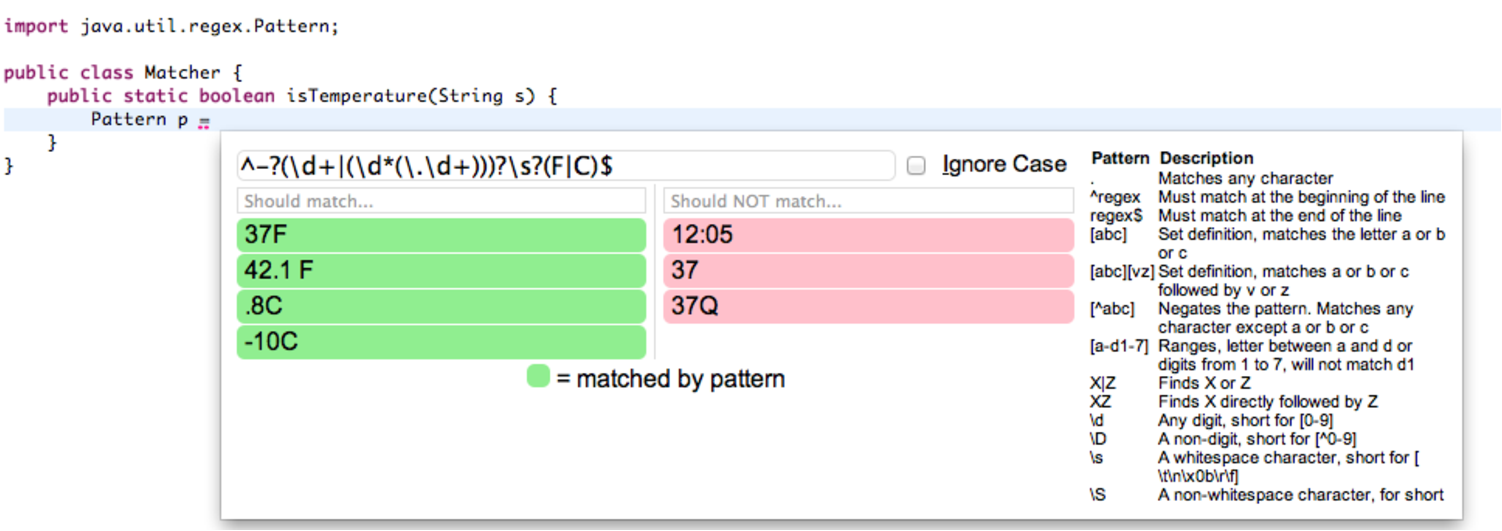
\includegraphics[scale=.55]{regex-palette.pdf}\\
% $\Downarrow$ \text{(pressing \textbf{Enter})}\\
% 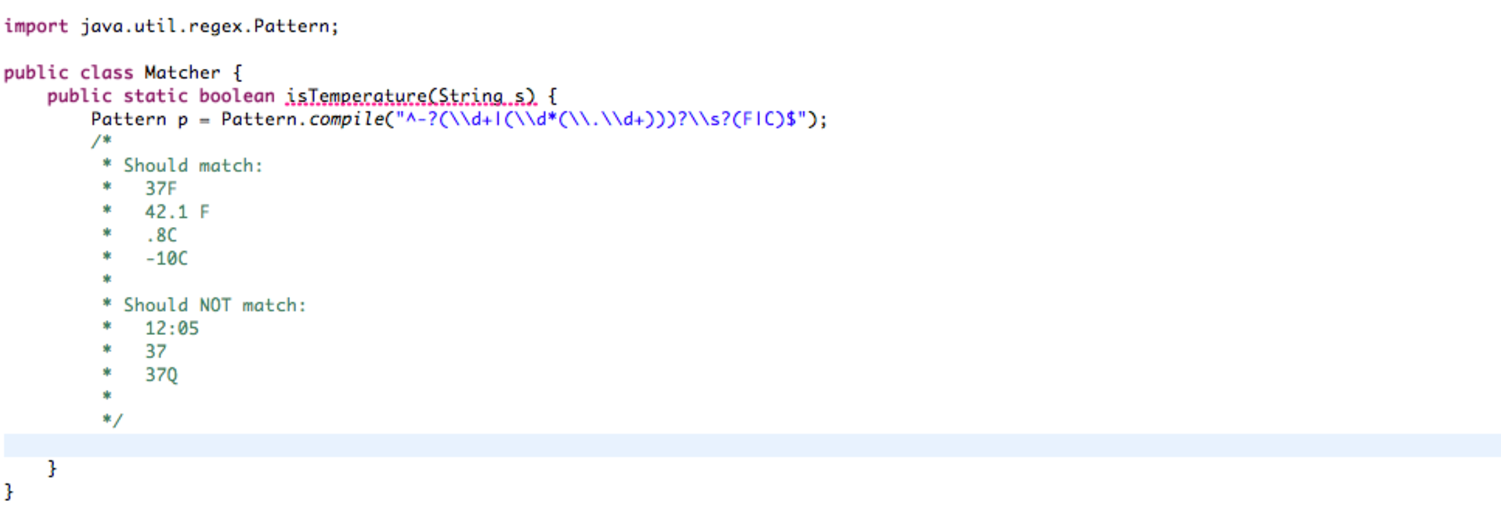
\includegraphics[scale=.55]{regex-code-generated.pdf}
% \end{center}
% \vspace{-20px}
% \caption{An example of type-specific editor services, here shown for Java.}
% \label{fig:regex-palette}
% %\vspace{-10px}
% \end{figure}

%In a conventional \emph{monolithic} programming system, support for each of these features would need to be built into the language and tools. 

To express the concrete syntax of patterns, regular expression library providers usually provide a utility function that transforms strings to patterns. As just mentioned, there  may be many implementations of the \lstinline{PATTERN} signature, so the standard approach is to define a \emph{parameterized module} (a.k.a. \emph{functor} in SML) defining utility functions generically:

\begin{lstlisting}[numbers=none]
module PatternUtil(P : PATTERN)
  fun parse(s : string) : P.t
    (* ... pattern parser here ... *)
\end{lstlisting}
This allows the client of any module \lstinline{P : PATTERN} to use the following definitions:
\begin{lstlisting}[numbers=none]
module PU = PatternUtil(P)
let pattern = PU.parse
\end{lstlisting}
to construct patterns like this:
\begin{lstlisting}[numbers=none]
pattern "SSTRA|T|G|CESTR"
\end{lstlisting}
 %Again, none of our goals are comprehensively achieved.
This approach is imperfect for several reasons:
\begin{enumerate} 
\item Our first problem is syntactic: string escape sequences conflict syntactically with pattern escape sequences. For example, the following will not be well-formed:
\begin{lstlisting}[numbers=none,mathescape=|]
let ssn = pattern "SSTR\d\d\d-\d\d-\d\d\d\dESTR"
\end{lstlisting}
When compiling an analagous expression using \verb|javac|, we encounter the error message \verb|error: illegal escape character|.\footnote{When compiling an analagous expression using SML of New Jersey (SML/NJ), we encounter the seemingly inexplicable error message \texttt{Error: unclosed string}.} In a small lab study, we observed that this error was common, and nearly always initially misinterpreted by even experienced programmers who hadn't used regular expressions recently \cite{Omar:2012:ACC:2337223.2337324}. The inelegant workaround is to  double backslashes:
\begin{lstlisting}[numbers=none]
let ssn = pattern "SSTR\\d\\d\\d-\\d\\d-\\d\\d\\d\\dESTR"
\end{lstlisting}

Some languages, anticipating such modes of use, build in special string forms that leave escape sequences uninterpretted. For example, Ocaml allows the following, which is perhaps more acceptable:
\begin{lstlisting}[numbers=none]
let ssn = pattern {rx|SSTR\d\d\d-\d\d-\d\d\d\dESTR|rx}
\end{lstlisting}

\item The next problem is that pattern parsing does not occur until the pattern is evaluated at run-time. For example, the following malformed pattern will only trigger an error when this expression is evaluated during the full moon: %Achieving this goal is an explicit goal of this proposal, so we are obviously not happy with this.

\begin{lstlisting}[numbers=none]
case moon_phase
  Full => pattern "SSTR(GCESTR" (* malformedness not statically detected *)
  _ => (* ... *)
\end{lstlisting}
Such issues can sometimes be found via testing, but empirical data gathered from open source projects suggests that there remain many malformed regular expression patterns that are not detected by a project's test suite ``in the wild'' \cite{spishak2012type}. 

We might instead attempt to treat the well-formedness of patterns constructed from strings as a static verification condition. Statically proving that this condition holds throughout a program is wildly difficult to automate in general, because it involves reasoning about arbitrary dynamic behavior. In the example above, we must know that the variable \lstinline{pattern} is equivalent to the function \lstinline{PU.pattern}. Moreover, if the argument were not written literally, e.g. we had written \lstinline{strconcat "SSTR(GESTR" "SSTRCESTR"}, we would need to be able to establish that this is equivalent to the string above. It is simple to come up with arbitrarily more complex examples that thwart any putative decision procedure, particularly for patterns that are dynamically constructed based on input to the program (further discussed below).

Parsing patterns at run-time also incurs a performance penalty. To avoid incurring it every time the pattern is encountered (e.g. for each item in a very large dataset), one must be careful to stage the computation appropriately, or use an appropriately tuned caching strategy. %This too is difficult if a portion of the pattern is dynamically generated. % Regular expressions are often used across large datasets in scientific applications, so the absolute peformance penalty can be non-trivial.

\item The final problem is that using strings to construct patterns encourages programmers to use string concatenation inappropriately to construct patterns derived from user input. For example, consider the following function:
\begin{lstlisting}[numbers=none,escapechar=|]
fun example_bad(name : string)
  pattern (name ^ "SSTR: \\d\\d\\d-\\d\\d-\\d\\d\\d\\dESTR")
\end{lstlisting}
The (unstated) intent here is to treat \lstinline{name} as a sub-pattern matching only itself, but this is not the observed behavior when \lstinline{name} contains special characters that mean something else in patterns. The correct code again resembles abstract syntax: 
\begin{lstlisting}[numbers=none]
fun example_fixed(name : string)
  P.Seq(P.Str(name), P.Seq(pattern "SSTR: ESTR", ssn)) (* ssn as above *)
\end{lstlisting}

In applications that query sensitive data, failures of this variety can lead to \emph{injection attacks}.  These are observed to be both common and catastrophic from the perspective of security \cite{owasp2013}. The attack vector above was, of course, the fault of the programmer using a flawed heuristic, so it could have been avoided with sufficient discipline. 
The problem is again that it is difficult to detect violations of this discipline automatically. Both functions above have the same type and behave identically at many inputs, particularly those that would be expected during typical executions of the program (i.e. alphabetic names), so testing often misses the problem. Formally proving that such problems do not arise involves reasoning about complex run-time data flows. 

 %Ideally, our library would be able to make it more difficult to inadvertently introduce subtle security bugs like this.
\end{enumerate}
% \begin{enumerate}
% \item \textbf{Conventional Concrete Syntax.} Patterns must be written in exactly the conventional manner, shown in blue below. Curly braces serve as an ``unquote'' form to splice one pattern into another:
% \begin{lstlisting}[numbers=none]
% let N : Pattern = /SURLA|T|G|CEURL/
% let BisI : Pattern = /SURLGC{EURLNSURL}GCEURL/
% let twoDigits : Pattern = /SURL\d\dEURL/\end{lstlisting}

% %The choice of delimiter, i.e. matching forward slashes here, is not important.
% %The cognitive load of reading and writing patterns is low and patterns are parsed once at compile-time. 
% \item \textbf{Compile-Time Parsing.} Pattern parsing must occur at compile-time, i.e. it must not incur run-time cost and malformed patterns, e.g. \lstinline{/SURLGC(EURL/}, must result in {compile-time} errors no matter where they appear in the program. 
% \item \textbf{Security By Default.} Strings must not be treated as patterns, nor used idiomatically to construct patterns. For example, the function below must be ill-typed because \lstinline{name} is not of type \lstinline{Pattern}:
% \begin{lstlisting}[numbers=none]
% fun example(name : string) : Pattern
%   let twoDigits : Pattern = /SURL\d\dEURL/
%   /SURL{EURLnameSURL}: {EURLtwoDigitsSURL}EURL/
% \end{lstlisting}
%     It is also acceptable for \lstinline{example("SSTR[a-z]ESTR")} to be equivalent to \lstinline{/SURL\[a-z\]: \d\d/}, i.e. strings are treated as patterns matching only themselves. 
% It is \emph{not} acceptable for \lstinline{example("SSTR[a-z]ESTR")} to be equivalent to \lstinline{/SURL[a-z]: \d\d/}. 

%     This is a security issue because if \lstinline{name} is derived from user input, such confusion could lead to \emph{injection attacks}, which are both common and catastrophic when using regular expression libraries that fail to achieve these goals, discussed below \cite{owasp2013}. 
%   %\item A more advanced semantics might ensure that out-of-bounds backreferences to a captured group do not occur \cite{spishak2012type}. For example, we would want \verb|BisI|, above, to have the more precise type \lstinline{Pattern(1)}, i.e. a pattern with one captured group. 
% % \end{enumerate}
% %When an error is found, an intelligible error message is provided.
% %\item An \textbf{implementation} that partially or fully compiles known regular expressions into the efficient internal representation that will be used by the regular expression matching engine (e.g., a finite automata \cite{Thompson:1968:PTR:363347.363387}) ahead of time. In most languages, this compilation step occurs at run-time, even if the pattern is fully known at compile-time, thereby introducing performance overhead into programs. If the developer is not careful to cache compiled representations, regular expressions used repeatedly in a program might be needlessly re-compiled on each use. %By performing this step ahead-of-time, these dangers can be avoided.
% %\item A range of \textbf{editor services} that support syntax highlighting for patterns, retrieval of relevant documentation, interactive testing, and pattern extraction from example strings have been shown to be helpful for programmers when working with complex regular expressions \cite{ACC_VLHCC}. An example of some of these is shown in Figure \ref{fig:regex-palette}: the editor service shown helps programmers generate correct code, here via the Java standard library's implementation of regular expressions (discussed below).
% \end{enumerate}
% Let us consider the ways that providers of regular expression libraries commonly choose to define the type \verb|Pattern|: as synonymous to \lstinline{string}, as a recursive sum type, or as an abstract type.

% \vspace{-5px}
% \paragraph{Patterns as Strings} The most na\"ive choice is to define \lstinline{Pattern} as synonymous to \lstinline{string}:

% \begin{lstlisting}[numbers=none]
% type Pattern = string
% \end{lstlisting}
% The only reason to consider this definition is that it allows us to approximate pattern syntax using standard string literal syntax:

% \begin{lstlisting}[numbers=none]
% let N : Pattern = "SSTRA|T|G|CESTR"
% \end{lstlisting}
% To splice one pattern into another, we can perform string concatenation:
% \begin{lstlisting}[numbers=none,escapechar=|]
% let BisI : Pattern = "SSTRGCESTR" ^ N ^ "SSTRGCESTR"
% \end{lstlisting}
% or use string interpolation (as in Scala or SML/NJ using quotation/antiquotation \cite{SML/Quote}):
% \begin{lstlisting}[numbers=none,mathescape=|]
% let BisI : Pattern = s"SSTRGC${ESTRNSSTR}GCESTR"
% \end{lstlisting}

% Though this comes close, goal 1 is not truly achieved because the syntax of strings can conflict with the syntax for patterns. 

% Goal 2 is not achieved because parsing occurs only at run-time when we match a string against a pattern (worse, every time we do so unless the implementation uses an effective caching strategy).

% Goal 3 is also not achieved because the following code typechecks:
% \begin{lstlisting}[numbers=none,mathescape=|]
% fun example_bad_1(name : string) : Pattern
%   let twoDigits : Pattern = "SSTR\\d\\dESTR"
%   s"SSTR${ESTRnameSSTR}-${ESTRtwoDigitsSSTR}"ESTR
% \end{lstlisting}
% but \lstinline{example_bad_1("SSTR[a-z]ESTR")} evaluates to \lstinline{"SSTR[a-z]-\\d\\dESTR"}.



% \paragraph{Patterns as Recursive Sums} A more semantically justifiable strategy is to define \lstinline{Pattern} as a recursive sum type  \cite{pfpl}. Verse supports these in the form of case types, which are analagous to datatypes in ML:

% \begin{lstlisting}[numbers=none]
% casetype Pattern
%   Empty
%   Str of string
%   Seq of Pattern * Pattern
%   Or of Pattern * Pattern
%   Star of Pattern  
% \end{lstlisting}

% More generally, we can hold the representation of patterns abstract while exposing an isomorphic interface to clients by defining an abstract type in a {module} opaquely ascribed the following {module type} (a.k.a. \emph{signature} in SML): % exposes the constructors and case analysis as functions:

% \begin{lstlisting}[deletekeywords={case},numbers=none]
% module type PATTERN
%   type t
%   val Empty : t
%   val Str : string -> t
%   val Seq : t * t -> t
%   val Or : t * t -> t
%   val Star : t -> t
%   val case : (
%     'a -> 
%     (string -> 'a) ->
%     (t * t -> 'a) ->
%     (t * t -> 'a) ->
%     (t -> 'a) ->
%     'a)
% \end{lstlisting}
% The client of any module \lstinline{P : PATTERN} can define \verb|Pattern| as synonymous to \verb|P.t|: 
% \begin{lstlisting}[numbers=none]
% type Pattern = P.t
% \end{lstlisting}



%The first one might not be found incorrect without rigorous testing with unexpected inputs. Goal 3 expresses the ideal of designing a language where security does not require considering such subtle issues extralinguistically.%This is precisely why injection attacks are so difficult to detect.

% The dialect of Standard ML implemented by SML/NJ, recognizing that directly using constructors is often less than ideal, provides a facility for quotation/antiquotation \cite{SML/Quote}, which if introduced into Verse could be used as follows:
% \begin{lstlisting}[numbers=none,escapechar=|,mathescape=|]
% fun example(p : string)
%   let twoDigits = P.qparse `SQT\d\dEQT`
%   P.qparse `SQT^(EQTP.Str(p)SQT)-^(EQTtwoDigitsSQT)EQT`
% \end{lstlisting}

% Here, backticks are used to indicate a quoted term within which carets serve as an antiquote operator. This still represents a  compromise against goal 1. The most serious problem is that, once again, parsing does not occur until run-time. There are also  conflicts between quotation syntax and pattern syntax, i.e. \verb|^| conventionally means character set negation inside patterns, which conflicts with antiquotation here. This mechanism also does not support antiquotation at more than one type, so we could not define the antiquote operator to insert the \verb|Str| constructor automatically, as suggested in goal 3. %For syntax that necessary involves antiquotation at multiple types (e.g. concrete syntax for a programming language with multiple syntactic sorts, HTML which might include Javascript and CSS, and others), this 

\subsection{Existing Approaches}\label{sec:syntax-existing} These difficulties with string-oriented approaches to concrete syntax are not particular to regular expression patterns, but rather arise in many similar scenarios, motivating much research on reducing the need for run-time string parsing \cite{Bravenboer:2007:PIA:1289971.1289975}. Existing approaches take one of two approaches: \emph{syntax extension} or \emph{static term rewriting}. 

\subsubsection{Syntax Extension}
One common approach is to use a system that allows users to directly extend the syntax of a language with new derived syntax, in this case for patterns.

The simplest such systems are those where each new syntactic form is described by a single rewrite rule. For example, the external language of Coq (called Gallina) includes such a system \cite{Coq:manual}. A formal account of such systems has been developed by Griffin \cite{5134}. Unfortunately, these systems are not able to express pattern syntax in the conventional manner. For example, sequences of characters  can only be parsed as identifiers using these systems, rather than as characters in a pattern. Syntax extension systems based on context-free grammars like  Sugar* \cite{erdweg2013framework}, Camlp4 \cite{ocaml-manual} and many others are more expressive, and would allow us to directly introduce pattern syntax into our core language's grammar.

However, this is a perilous approach because none of the systems described thusfar guarantee \emph{syntactic composability}, i.e. as the Coq manual states: ``mixing different symbolic notations in [the] same text may cause serious parsing ambiguity''. If another library provider used similar syntax for a different variant of regular expressions, or for an entirely unrelated abstraction, then a client could not simultaneously use both libraries in the same scope. Properly considered, every combination of extensions introduced by one of these mechanisms creates a \emph{de facto} derived syntactic dialect of the language. % Resolving such parsing amibiguities is left to each client of the library. 

In response to this problem, Schwerdfeger and Van Wyk have developed a modular analysis that accepts only grammar extensions that use a unique starting token and satisfy some subtle conditions on follow sets of base language non-terminals \cite{conf/pldi/SchwerdfegerW09}. Such extensions can be used together in any combination. However, simple starting tokens like \lstinline{pattern} cannot be guaranteed to be globally unique, so we would need to use a more verbose starting token like \lstinline{edu_cmu_verse_rx_pattern}. There is no principled way to define local abbreviations for starting tokens because this mechanism is language-external.

Putting this issue aside, we must now decide how our newly introduced derived forms elaborate to forms in our base grammar. In this case, because we are using a modular encoding of patterns, we must first decide which module the desugaring will use. Clearly, simply assuming that a module identified as \lstinline{P} satisying \lstinline{PATTERN} is in scope is a brittle solution. Indeed, we should expect that the extension mechanism actively prevents such capture of specific variable names to ensure that variables (including module variables) can be freely renamed. Such a \emph{hygiene discipline} is well-understood when performing term-to-term rewriting (discussed below) or in simple rewrite systems like those found in Coq. For more flexible mechanisms, the issue is a topic of ongoing research (none of the grammar-based mechanisms described above enforce hygiene).

Putting aside the question of hygiene as well, we can address the problem by requiring that the client explicitly identify the module the desugaring should use:
\begin{lstlisting}[numbers=none]
let ssn = edu_cmu_verse_rx_pattern P /\d\d\d-\d\d-\d\d\d\d/
\end{lstlisting}
For patterns constructed compositionally, we can define \emph{splicing} syntax for both strings and other patterns:
\begin{lstlisting}[numbers=none,escapechar=|]
fun example_syn(name : string)
  edu_cmu_verse_rx_pattern P /@name: %ssn/
\end{lstlisting}
The body of this function elaborates to the body of \lstinline{example_fixed} as shown above. Had we mistakenly used the pattern splicing prefix, \lstinline{%name}, rather than the string splicing prefix, \lstinline{@name}, we would get a static type error, rather than a silent security vulnerability.

Such syntax extension approaches suffer from a paucity of direct reasoning principles. Given an unfamiliar piece of syntax, there is no simple method for determining what type it will have, or even for identifying which extension determines its desugaring, causing difficulties for both humans (related to code comprehension) and tools.

\subsubsection{Term Rewriting}
An alternative approach is to leave the concrete syntax of the language fixed, but repurpose it for novel ends using a \emph{local term-rewriting system}. Among the earliest examples is the LISP macro system \cite{Hart63a}. This system was later refined, notably in Scheme and its dialects to better support reasoning compositionally about the rewriting that is performed \cite{Kohlbecker86a}. In languages with a stronger static type discipline, variations on macros that restrict rewriting to a particular type and perform the rewriting in an explicitly staged manner have also been studied \cite{Herman10:Theory,ganz2001macros} and integrated into languages, e.g. MacroML \cite{ganz2001macros} and Scala \cite{ScalaMacros2013}. 

The most immediate problem with using these in our example is that we are not aware of any such statically-typed macro system that integrates cleanly with an ML-style module system. However, let us imagine a macro system that would allow us to repurpose string syntax  as follows:
\begin{lstlisting}[numbers=none]
let ssn = pattern P {rx|SSTR\d\d\d-\d\d-\d\d\d\dESTR|rx}
\end{lstlisting}

Here, \lstinline{pattern} is a macro parameterized by a module \lstinline{P : PATTERN}. It statically parses the provided string literal (which must still be written using an Ocaml-style literal here) to generate an elaboration, at type \lstinline{P.t}. 

For patterns that are constructed compositionally, we need to get more creative. For example, we might repurpose the infix operators that the language provides for other purposes:

\begin{lstlisting}[numbers=none,escapechar=|]
fun example_macro(name : string)
  pattern P (name ^ "SSTR: ESTR" + ssn)
\end{lstlisting}

This does not give us syntax that is quite as clean and clear as the syntax available using syntax extensions, but it does address a number of its deficiencies: there cannot be syntactic conflicts (because the syntax is not extended), we can define macro abbreviations because macros are integrated into the language, there is a hygiene discipline that guarantees that the elaboration will not capture variables inadvertently, and there is a typing discipline (i.e. we need not determine the elaboration to know what type it will have). 

% \begin{enumerate}
% \item Given an unfamiliar piece of syntax, there is no simple method for determining what type it has, or to identify which extension determines its desugaring, hindering code comprehension.
% \item It requires that the syntax be expressed as a grammar that can be consumed by a particular parser generator. Not all syntax  is most naturally expressed in this way, but there is no way to use a ``hand-rolled'' parser.
% \end{enumerate}

\subsection{Contributions}\label{sec:syntax-contributions}
We propose a new primitive, the \textbf{typed syntax macro} (TSM), that combines the flexibility of syntax extensions with the reasoning guarantees of statically-typed macros, and show how to integrate it into a language with an ML-style module system, addressing all of the problems described above. We then introduce \textbf{type-specific languages} (TSLs), which leverage local type inference to control TSM dispatch. This further decreases syntactic cost (which is, of course, the entire purpose of this exercise). The result is that derived syntax defined using TSLs  approaches the cost of derived syntax built in primitively.

\subsubsection{Typed Syntax Macros (TSMs)}
%A typed syntax macro is invoked by applying it to a \emph{delimited form}, which can contain  arbitrary syntax in its \emph{body}.  
As our first example, consider the following concrete term:
\begin{lstlisting}[numbers=none]
pattern P /SURLA|T|G|CEURL/
\end{lstlisting}
Here, a parameterized TSM \lstinline{pattern} is applied to a module parameter, \lstinline{P}, and a {delimited form}, \lstinline{/SURLA|T|G|CEURL/}. Based on the body of the delimited form, i.e. the characters between the delimiters, the TSM statically computes an elaboration to the following {base external form}:

% import cs.cmu.edu/~wyvern/regex as R
% let syntax pattern = R.pattern
% let module P = R.P
% The first line imports our top-level regular expression module (identified uniquely by a URI) and binds a shorter name, \lstinline{R}, to it. The second line binds a local name to the  TSM named \lstinline{pattern} that \lstinline{R} exports. The third line gives a shorter name, \lstinline{P}, to the module \lstinline{R.P : R.PATTERN}, as defined previously. The fourth line then applies \lstinline{pattern} to this module parameter and a form delimited by forward slashes. This causes it to elaborate \emph{statically} to the following base form:
\begin{lstlisting}[numbers=none]
P.Or(P.Str "SSTRAESTR", P.Or(P.Str "SSTRTESTR", P.Or(P.Str "SSTRGESTR", P.Str "SSTRCESTR")))
\end{lstlisting}
The parameterized TSM \lstinline{pattern} is defined as shown below:
\begin{lstlisting}[numbers=none]
syntax pattern(P : PATTERN) at P.t
  fn (ps : ParseStream) => (* pattern parser here *)
\end{lstlisting}
We declare a module parameter (calling it \lstinline{P} here is unimportant, i.e. the TSM can be used with \emph{any} module satisfying module type \lstinline{PATTERN}), which is bound in the scope of the type clause \lstinline{at P.t}. This clause  guarantees that all elaborations successfully generated by this TSM will be of type \lstinline{P.t}. Elaborations are generated by the static action of the parse function defined in the indented block on the next line. The parse function must be of type \lstinline{ParseStream -> Exp}, where the type \lstinline{ParseStream} gives the function access to the \emph{body} of the delimited form (in blue above) and the type \lstinline{Exp} is a case type that encodes the abstract syntax of the base language (i.e. the Verse EL). Both types are defined in the Verse \emph{prelude}, which is a set of definitions available ambiently.

In positions where the type is known, e.g. due to a type ascription or at the argument position of a function call, the module parameter \lstinline{P} can be inferred:
\begin{lstlisting}[numbers=none]
let N : P.t = pattern /SURLA|T|G|CEURL/
\end{lstlisting}

TSMs can be partially applied and abbreviated using a let-binding style mechanism:
\begin{lstlisting}[numbers=none]
let syntax pat = pattern P 
let ssn = pat /SURL\d\d\d-\d\d-\d\d\d\dEURL/
\end{lstlisting}

TSMs can treat portions of the body of the delimited form as a spliced base language term, to support splicing syntax:
\begin{lstlisting}[numbers=none]
fun example_tsm(name: string)
  pat /SURL@EURLnameSURL: %EURLssn/
\end{lstlisting}
A hygiene mechanism ensures that only those portions of the elaboration derived from such spliced terms can refer to variables in the surrounding scope, preventing inadvertent variable capture by the elaboration. In other words, the generated elaboration must be context-independent.

\paragraph{Formalization} To give a flavor of the formal specification underlying TSMs, let us look at the rule for handling TSM invocation in a synthetic position. 
\begin{mathpar}
\inferrule[syn-aptsm]{
    \Delta \vdash s ~@~ \sigma~\{\iota_\text{parser}\}\\
    \mathbf{parsestream}(body) = \iota_\text{ps}\\
    \iota_\text{parser}(\iota_\text{ps}) \Downarrow \iota_\text{elab}\\
    \iota_\text{elab} \uparrow e_\text{elab}\\\\
    \Delta; \Gamma; \emptyset; \emptyset \vdash e_\text{elab} \Leftarrow \sigma \leadsto \iota
}{
    \Delta_\text{out}; \Gamma_\text{out}; \Delta; \Gamma \vdash \mathbf{invoketsm}(s; body) \Rightarrow \sigma \leadsto \iota
}
\end{mathpar}
Note that the judgement forms are  slightly simplified in that they omit various contexts relevant only to other Verse primitives. We include only \emph{typing contexts}, $\Gamma$, which map variables to types, and \emph{type abstraction contexts}, $\Delta$, which track universally quantified type variables (both in the standard way). The premises have the following purposes:
\begin{enumerate}
\item The first premise can be pronounced ``Under $\Delta$, TSM expression $s$ is a TSM at type $\sigma$ with parser $\iota_\text{parser}$''. Application of a parameterized TSM to its parameters is handled by this judgement (not shown).
\item The second premise creates a parse stream, $\iota_\text{ps}$, from the body of the delimited form.
\item The third premise applies the parser to the parse stream to generate an encoding of the elaboration, $\iota_\text{elab}$.
\item The fourth premise decodes $\iota_\text{elab}$, producing the elaboration $e_\text{elab}$.
\item The fifth premise validates the elaboration by analyzing it against the type $\sigma$ under an empty context. The \emph{current} typing and kinding contexts are ``saved'' for use when a spliced term is encountered during this process by setting them as the new \emph{outer contexts}.

Variables in the outer contexts cannot be used directly by the elaboration, e.g. they are ignored by the (syn-var) rule:
\begin{mathpar}
\inferrule[syn-var]{ }{
    \Delta_\text{out}; \Gamma_\text{out}; \Delta; \Gamma, x : \sigma \vdash x \Rightarrow \sigma \leadsto x
}
\end{mathpar}
The outer contexts are switched back in only when encountering a spliced expression, which is marked:
\begin{mathpar}
\inferrule[syn-spliced]{
    \emptyset; \emptyset; \Delta_\text{out}; \Gamma_\text{out} \vdash e \Rightarrow \sigma \leadsto \iota
}{
    \Delta_\text{out}; \Gamma_\text{out}; \Delta; \Gamma \vdash \mathbf{spliced}(e) \Rightarrow \sigma \leadsto \iota
}

\inferrule[ana-spliced]{
    \emptyset; \emptyset; \Delta_\text{out}; \Gamma_\text{out} \vdash e \Leftarrow \sigma \leadsto \iota
}{
    \Delta_\text{out}; \Gamma_\text{out}; \Delta; \Gamma \vdash \mathbf{spliced}(e) \Leftarrow \sigma \leadsto \iota
}
\end{mathpar}
For example, the elaboration generated in \lstinline{example_tsm} above would be:
\begin{lstlisting}[numbers=none]
P.Seq(P.Str(spliced(name)), P.Seq(P.Str ": ", spliced(ssn)))
\end{lstlisting}
\end{enumerate}

We will give a more complete account of all of these judgements later.
\subsubsection{Type-Specific Languages (TSLs)}
To further lower the syntactic cost of using TSMs, Verse also  supports \emph{type-specific languages} (TSLs), which allow library providers to associate a TSM directly with a declared type. For example, a module \lstinline{P} can associate \lstinline{pattern} with \lstinline{P.t} as follows:
\begin{lstlisting}[numbers=none]
module P : PATTERN with syntax pattern at t
  type t = (* ... *)
  (* ... *)
\end{lstlisting}

 Local type inference then determines which TSM is applied when analyzing a delimited form not prefixed by a TSM name. For example, the following is equivalent to the above:
\begin{lstlisting}[numbers=none]
fun example_tsl(name : string) : P.t
  /SURL@EURLnameSURL: %EURLssn/
\end{lstlisting}

As another example, we can use TSLs to express derived list syntax. For example, if we use a case type, we can declare the TSL directly upon declaration as follows:
\begin{lstlisting}[numbers=none]
casetype list('a) {
  Nil
  Cons of 'a * list('a)
} with syntax
  fn (body : ParseStream) => (* ... comma-delimited spliced exps ... *)
\end{lstlisting}
Together, this allows us to write a list of patterns like this:
\begin{lstlisting}[numbers=none]
let x : list(P.t) = [/SURL\dEURL/SHTML, EHTML/SURL\d\dEURL/SHTML, EHTML/SURL\d\d\dEURL/]
\end{lstlisting}

\subsection{Timeline}\label{sec:syntax-timeline}
We have described and formally specified TSMs in a recently published paper \cite{sac15}, and TSLs in a paper last year \cite{TSLs}, both in the context of the Wyvern language. In the context of Verse, there are some changes that need to be made in the formalization. In particular, neither paper covered integration with an ML-style module system. We plan to complete this in the course of writing the dissertation. 

% \subsection{Typed Syntax Macros (and Type-Specific Languages)}
% Consider the following \emph{recursive case type}, which encodes the tree structure of HTML documents (we will see how case types are themselves library constructs later):
% \begin{lstlisting}[numbers=none]
% casetype HTML
%   Empty
%   Seq of HTML * HTML
%   TextNode of string
%   H1Element of Attributes * HTML (* Attributes not shown *)
%   (* ... *)
% \end{lstlisting}
% We can introduce values of this type by applying one of these declared constructors to data of the corresponding type. For example, here is a function that creates a heading given a string (assuming the variable \lstinline{empty_attrs : Attributes} is in scope, not shown):
% \begin{lstlisting}[numbers=none]
% fun make_heading(x : string) -> HTML
%   H1Element(empty_attrs, TextNode(x))
% \end{lstlisting}
% The same function can be written using more idiomatic HTML syntax via a TSM as follows:
% \begin{lstlisting}[numbers=none]
% fun make_heading_tsm(x : string)
%   html `SHTML<h1><%EHTMLxSHTML></h1>EHTML`
% \end{lstlisting}
% Here, \lstinline{html} identifies a TSM defined as below:
% \begin{lstlisting}[numbers=none]
% syntax html for HTML
%   fn (body : ParseStream) -> Exp => (* ... *)
% \end{lstlisting}
% The function in the indented block is invoked {statically} to generate an \emph{elaboration} based on the {body} of the \emph{delimited form} provided to the TSM, here \lstinline{SHTML<h1><%EHTMLxSHTML></h1>EHTML}, 
% for subsequent typechecking and translation to the Verse IL. In this example, the elaboration generated is equivalent to the one shown above in \lstinline{make_heading}. Both \lstinline{ParseStream}, which provides access to the body as a stream of characters, and \lstinline{Exp}, which encodes the abstract syntax of the Verse EL, are types defined in the Verse \emph{prelude}, which is simply a collection of definitions loaded before all others. The implementation of this parse function is not particularly interesting, so we omit it here. We will discuss how generating this function from a declarative grammar specification is itself a mode of use of TSMs later.

% Notice that a portion of the body, indicated in black for clarity, is treated as a \emph{spliced expression}. The TSM determines what syntactically distinguishes spliced expressions (here, the delimiters \lstinline{<%} and \lstinline{>} around an identifier or, not shown, \lstinline{<%>} and \lstinline{</%>} around an expression). 
% Verse only specifies the delimiters that can be used to transition from the expression language to the TSM body (here, we used backticks, but Verse supports several others, including \emph{layout delimiters}, which we will discuss later). This ensures that syntactic conflicts cannot arise by construction and localizes reasoning about syntactic ambiguity to each TSM, without incurring substantial syntactic cost.

% The semantics includes an \emph{elaboration validation} step that maintains a \emph{hygiene discipline} by ensuring that the elaboration does not make any assumptions about the context around the TSM application. In particular, only portions of the elaboration derived from spliced expressions can refer to variables in the surrounding context. Moreover, by requiring that the TSM provide a type annotation, it maintains a \emph{typing discipline}. For example, due to the type annotation on the definition of \lstinline{html} above, clients can assume that all successful applications of the TSM will elaborate to a term of type \lstinline{HTML}, without needing to reason about the elaboration logic itself. Not shown here, this annotation can be parameterized by types as well as modules. Because the Verse module system is borrowed directly from ML,  this means that TSMs can be used to define derived syntax valid for all instances of an abstract type. We will discuss this after motivating it with another example in Section \ref{sec:syntax}.

% To decrease the syntactic cost of applying a TSM even further (controlling syntactic cost being, of course, the very purpose of TSMs), Verse can often locally infer these parameters. Moreover, when a type is declared, Verse allows the library provider to designate one TSM as its \emph{type-specific language} (TSL). Clients can then omit mention of this TSM entirely in positions where an expression of that type is expected. For example, if \lstinline{html} was designated as the TSL for \lstinline{HTML}, then we could have written the function above equivalently as:
% \begin{lstlisting}[numbers=none]
% fun make_heading_tsl(x : string) -> HTML
%   'SHTML<h1><%EHTMLxSHTML%></h1>EHTML'
% \end{lstlisting}

%These mechanisms are one reason why we specify Verse by a bidirectionally typed elaboration semantics.

\section{Modularly Metaprogrammable Type Structure}\label{sec:metamodules}
The Verse EL also does not build in substantial type structure. Only functions are built in directly. The type structure of case types (shown in use above), tuples, records, objects and other more esoteric constructs that we will describe later can all be expressed as modes of use of \emph{metamodules} (which are distinct from, though conceptually related to, \emph{modules}). 

The remainder of this section is organized like Section \ref{sec:syntax}. We begin with an example of type structure that cannot be expressed in languages like ML directly in Sec. \ref{sec:metamodules-example}, then show how existing approaches are insufficient in Sec. \ref{sec:metamodules-related}. Then we outline our approach in Sec. \ref{sec:metamodules-solution} and conclude with a timeline for remaining work in Sec. \ref{sec:metamodules-timeline}. 

\subsection{Motivating Example: Labeled Products and Regular Strings}\label{sec:metamodules-example}
As a simple introductory example, let us consider \emph{labeled products} and \emph{regular strings}. In Verse, a simple labeled product type classifying conference papers can be defined like this:
\begin{lstlisting}[numbers=none]
let type Paper = lprodtype {SPCT
  title : EPCTrstring /SURL.+EURL/
   SPCTconf : EPCTrstring /SURL([A-Z]+) (\d\d\d\d)EURL/
}
\end{lstlisting}
The first row is labeled \lstinline{title} and specifies the regular string type \lstinline{rstring /SURL.*EURL/}. Regular string types classify values that behave as strings known to be in the regular language specified by the regular expression given as the type parameter. Here, we have that paper titles must be non-empty strings. The second row is labeled \lstinline{conf} and specifies a regular string type with two parenthesized groups, corresponding to the conference abbreviation and the year.
The \lstinline{let type} construction defines a type synonym, \lstinline{Paper}. Alternatively, we could have used the following construction to declare \lstinline{Paper} \emph{generatively}:
\begin{lstlisting}[numbers=none]
lprodtype Paper {
  SPCTtitle : EPCTrstring /SURL.+EURL/
   SPCTconf : EPCTrstring /SURL([A-Z]+) (\d\d\d\d)EURL/
}
\end{lstlisting}
The difference is in how type equality is handled. Two labeled product types with the same signature are equal, unless declared generatively, in which case type equality is nominal.

In either case, we can introduce a value of type \lstinline{Paper} in an analytic position in one of two ways. We can omit the labels:
\begin{lstlisting}[numbers=none]
let exmpl : Paper = {"SUSAn Example PaperEUS"SCSS, ECSS"SUSEXMPL 2015EUS"}
\end{lstlisting}
Alternatively, we can include them explicitly for clarity:
\begin{lstlisting}[numbers=none]
let exmpl : Paper = {SCSStitle => ECSS"SUSAn Example PaperEUS"SCSS, conf => ECSS"SUSEXMPL 2015EUS"}
\end{lstlisting}

We can then project a row out of such a value using the row projection operator:
\begin{lstlisting}[numbers=none]
let exmpl_conf = # `SNATconfENAT exmpl 
\end{lstlisting}
Here, \lstinline{#} is an operator parameterized by a static label, written literally \lstinline{`SNATconfENAT}, and taking one argument, \lstinline{exmpl}. 

We can also project captured groups out of a regular string using the \lstinline{#group} operator, which is parameterized by a group index:
\begin{lstlisting}[numbers=none]
let exmpl_conf_name = #group 0 exmpl_conf
\end{lstlisting}

The variable \lstinline{exmpl_conf_name} has type \lstinline{rstring /SURL[A-Z]+EURL/}.

Both labeled products and regular strings support a number of other operations. For example, labeled products can be concatenated (with any common rows updated with the value on the right):
\begin{lstlisting}[numbers=none]
let a : lprodtype {SPCTauthors : EPCTlist(rstring /SURL.+EURL/)} = {["SUSHarry Q. BovikEUS"]}
let exmpl_paper_final = lprod+ exmpl_paper a
\end{lstlisting}
We can drop a row as well:
\begin{lstlisting}[numbers=none]
let exmpl_paper_anon = lprod- exmpl_paper_final `SNATauthorsENAT
\end{lstlisting}

\subsection{Existing Approaches}\label{sec:metamodules-related}
\subsubsection{Records and Tuples}
Recall that Verse builds in only nullary and binary products into its internal language, so the type structure described above for labeled products  is not directly expressible using IL primitives. If we weaken slightly our insistence on minimalism and built in record/tuple types, as in other functional languages, we have  options that get close to (but do not  exactly achieve) this type structure. In particular, unlike labeled product types, record types are identified up to row reordering. Using a record with the same row labels would prevent us from omitting the labels and relying on positional information when introducing a value of record type in an analytic position, as we did with type \lstinline{Paper} above. %If we instead use an unlabeled product type (which in ML is actually a record type with numeric labels, which are omitted syntactically), we lose the ability to use labels in the elimination form. 

One workaround is to replace each labeled product type in the program with a record type with row labels tagged by position (recovering the type disequality we seek to express with labeled product types) and conversion functions from the corresponding unlabeled product type and untagged record type to this type. 
This partially recovers some of the syntactic cost we seek, but introduces much additional  boilerplate as well as run-time cost. We are interested in such issues, so this is not an entirely satisfying solution. % In any case, records, tuples and labeled tuples are all library constructs in Verse. 
Moreover, this still does not give us support for the extra operations, like concatenation,  shown above.

\subsubsection{Refinement Types}
For regular strings, one could instead use standard strings (which themselves may be lists or vectors of characters together with derived syntax), inserting run-time checks around introductory forms and into other operations (with one exception, discussed below). This would, of course,  weaken the static semantics and add both syntactic and run-time cost. To recover the static guarantees of regular strings, we could treat membership of a string in a specified regular language as a static verification condition, moving the logic governing regular string types out of the language and into an external \emph{refinement type system} \cite{Freeman91}. 

One problem with this approach is that there is no direct analog to the group projection operator described above. The static and dynamic semantics of this operator depend on information available only in the static type of the regular string (i.e. the position of the captured group). Refinement types are strictly a layer above the language, and thus cannot affect its dynamic semantics.

A related problem is that there is no feasible way to use refinement types to introduce type disequalities that can later affect the internal representation of a value. All standard strings are represented uniformly. The fact that some value of type \lstinline{string} can be given a refined type \lstinline{rstring /A|B/} cannot be justification to locally alter its representation (e.g. to a single bit in this case). For regular strings, there may be limited benefit to doing this, but in general, this can have significant performance ramifications. For example, it is common to justify the omission of a primitive type of ``unsigned integers representable in 32 bits'' by the fact that this is ``merely'' a refinement of arbitrary precision integers, but in so doing one loses the ability to use a machine representation more suitable to this invariant.  %Refinement types cannot be used for this purpose without the possibility of conflict.
This is also the reason why one cannot viably do away with primitive record types by claiming that they are refinements of finite mappings.

Put another way, refinement types are useful when one only needs to make finer static distinctions within an existing type. When one needs to introduce new operators or type disequalities that have ``downstream'' impact, refinement types are not the right solution.%Refinement types are useful when no non-trivial operators need to be introduced into the language and the refinement has no impact on representation, but the type system itself must be extended in some way in more advanced situations.

\subsection{Contributions}\label{sec:metamodules-approach}

An important point is that labeled products, as well as other ``record-like'' constructs, can  be expressed by a \emph{type-directed translation} targeting our IL (and indeed, many compilers take advantage of facts like this to simplify the number of cases that must be considered downstream). %it is inaccurate to state that they are merely syntactic sugar over such a language. %Object systems are perhaps even more diverse across languages\todo{citation}. 
%Other dialects are justified by a desire to provide more special-purpose semantic constructs. For example, 
Substantially more sophisticated examples require at most only a very slightly more capable intermediate language (the IL of popular virtual machines, even those with flaws like ubiquitous \texttt{null} references, e.g. JVM or CIL bytecode, are also sufficient if used strictly as translation targets).

Metamodules introduce type and operator constructors parameterized by arbitrary \emph{static values} and metaprogrammatically express the logic governing their typechecking and  translation to the IL using the Verse \emph{static language} (SL). Metamodules are classified by \emph{metasignatures}. For example, let us consider the following metasignature:
\begin{lstlisting}
metasignature LPROD
  tycon c of LblTyList
  ana opcon intro_unlabeled
  ana opcon intro_labeled of LblList
  syn opcon # of Lbl
\end{lstlisting}\todo{reworking active tycons as metasignatures and metastructures is compelling, but I need to figure it out. will continue writing.}

% The semantics uses internal type abstraction to guarantee that metamodule providers can reason modularly about translation invariants, just as it uses external type abstraction to guarantee that module providers can reason modularly about representation invariants.%For example, a metamodule that expresses the type structure of records would introduce a type constructor  \texttt{record} parameterized by a static mapping from labels to types, and two operators: the introductory operator \texttt{intro}, parameterized by a list of row labels, and the row projection operator \texttt{prj}, parameterized by a row label. It might then choose to internally represent records by binary products, which the IL provides. Critically, the choice of internal representation is \emph{computed} based on each record type's parameter, and it is held abstract outside the metamodule using internal type abstraction, facilitating modular reasoning about translation invariants (just as external type abstraction facilitates modular reasoning about representation invariants in the module system). Metamodules like this can express many other constructs, including variants of records that support additional operations, labeled sums, object systems, constrained strings, typechecked operations on format strings like \texttt{printf} and typechecked foreign function interfaces. By using %This simplifies the Verse core language relative to the core languages of ML,  Scala and other comparable languages.


% These constructs, very generally summarized, give library providers \emph{metaprogrammatic control} over aspects of the \emph{external} (i.e. user-facing) textual syntax and type structure of Verse, respectively. This \emph{external language} (EL) is given meaning by type-directed translation to a minimal \emph{typed internal language} (IL), specified in a completely standard manner. In some ways, this style of language specification is comparable to a specification for the first stage of a type-directed compiler shifted ``one level up'' into the language and modularly reorganized. By \emph{metaprogrammatic control}, we mean that Verse exposes a \emph{static language} (SL) to library providers. Functions written in the SL, which we refer to as \emph{static functions}, are invoked by the external semantics to control certain aspects of parsing, elaboration, typechecking and translation. %This IL can be specified in a completely standard manner, but the user-facing \emph{external language} (EL) must be specified in a novel manner to support these constructs. 



%  %while imposing constraints in order to maintain strong metatheoretic guarantees, including the guarantee that these constructs can be reasoned about modularly and used together by clients in any combination, without the possibility of syntactic or semantic conflicts.\footnote{...other than simple naming conflicts, which must be handled by adopting appropriate naming conventions, e.g. based on URIs as in the Java ecosystem.} By \emph{metaprogrammatic}, we mean that Verse exposes a \emph{static language} (SL) to library providers. Functions written in the SL, which we refer to as \emph{static functions}, are invoked by the language to control certain aspects of parsing, elaboration, typechecking and translation to Verse's minimal typed internal language (IL), which is specified in the standard manner.% In a sense, Verse pulls machinery that is usually part of a compiler into the language specification so that it can give library providers greater control over it. 



% %Although metamodules are in some sense conceptually prior to TSMs, it will be  pedagogically useful for us to introduce TSMs first, in Sec. \ref{sec:syntax}, assuming temporarily that the core type structure is specified in the standard manner. We then show how metamodules can influence the type structure in Sec. \ref{sec:metamodules}.

% %This trend toward languages that are a growing hodge podge of constructs surrounded by an ecosystem of ``toy dialects'' can only be slowed by the development of mechanisms that are expressive enough to subsume large classes of existing constructs, pulling them out of the language definition and into modularly composable libraries. 




% % The ability to reason separately about libraries and import them freely is critical when constructing large software systems and participating in modern software ecosystems. If using a library requires a developer to directly modify the programming language they are using, detecting and resolving conflicts between constructs manually, then reestablish critical metatheoretic properties about the language followed by important invariants throughout their own code, the library will be essentially useless to them. 
% % %This means that it is difficult to construct large software systems and ecosystems from components written in different dialects. 
% % From this perspective, it is hardly surprising when software engineers avoid dialects and settle on a single common language, where they can rely on the guarantees provided by its module system to program ``in the large''. %The designers of these languages may slowly adopt the most generally useful new ideas. 
% % Unfortunately, this has left many useful constructs for programming ``in the small''  languishing in ``toy dialects''.% It is safe to say that in contemporary times, language dialects should be considered harmful. % It is little wonder that many programmers eschew esoteric language dialects in favor of languages that stopped evolving decades ago.

% % It is nearly always the case, however, that the dynamic semantics of these dialects can be defined by type-directed translation to the existing language. For example, ReactiveML builds in support for functional reactive programming, but its dynamic semantics can be implemented by type-directed translation to Standard ML \cite{mandel2005reactiveml}. In some cases, the semantics of the dialect are directly specified in this way. For example, F\# \cite{syme2012expert} introduces functional datatypes and the other constructs of the ML core language, defining them in terms of constructs available in the Common Intermediate Language (CIL), a class-based object-oriented language. Ocaml includes a class-based object system that can be defined by type-directed translation to Caml, a language building in little more than recursive product and sum types. 

% %{\Verse} aims to explore the polar opposite design philosophy: a core language designed to remain small and as unopinionated as possible. Rather than building in extensive syntax and type structure \emph{a priori}, it is organized around metaprogramming mechanisms that  %In other words, power is decentralized (though not completely, as we will discuss), while responsibility over metatheoretic guarantees remains ultimately in the hands of the language designer.

% Ensuring that the language specification is  metatheoretically well-behaved and, in particular, that the constructs that we introduce can be reasoned about modularly and used together in any combination is the primary challenge in this work. 
% For example, if we simply conceived of the language as being specified by a ``bag of forms and rules'' (like ``paper'' specifications of languages often appear) and let library providers introduce new forms and rules, as much of the related work does, one could easily cause syntactic conflicts, or introduce rules that violate type safety, interfere with invariants being maintained by rules defined in other libraries, or introduce undesirable forms of non-determinism into the semantics. %There is also the question of how to allocate finite syntactic resources. For example, as noted above, the design space around record types is large. If we allow libraries to explore this design space, which library gets to determine the meaning of a form like \lstinlinep{\{label1=e1, label2=e2\}}? 





%This suggests a need for language-integrated mechanisms that allow library providers to modularly express syntactic and semantic constructs of the sort that today require new dialects, allowing for perhaps some low-cost syntactic compromises.
%For example, it should be possible to express different record systems within a language specified like ML (or the simply typed lambda calculus). The challenge  is to give formal shape to these intuitions. %Our broad aim in this thesis is to design language mechanisms that take significant steps toward achieving this goal.

% \section{Contributions}
% \subsection{Verse}
% To provide a coherent vehicle for our contributions, we introduce a new programming language called Verse. Let us briefly review its organization. Syntactically, Verse has a layout-sensitive textual concrete syntax (i.e. newlines and indentation are meaningful). This choice is not fundamental to our proposed mechanisms, but it will be useful for cleanly expressing a class of examples that we will discuss later.  Semantically, Verse is organized into a \emph{module language} and a \emph{core language}. The module language is based directly on the Standard ML module language, with which we assume familiarity for the purposes of this proposal \cite{harper1997programming}. We will use it in an example in Section \ref{sec:syntax}. The core language is split into a user-facing \emph{external language} (EL) and a minimal \emph{typed internal language} (IL). The EL  is specified by a type-directed translation semantics targeting the much simpler IL. Notionally, this can be thought of as simply shifting the first stage of a type-directed compiler directly into the language specification \cite{tarditi+:til-OLD}. More specifically, we specify a {bidirectionally typed translation semantics}, i.e. one where a distinction is made between \emph{type analysis} (the type is an ``input'') and \emph{type synthesis} (the type is an ``output''), for reasons that we will return to later. 

% The main novelty is that the Verse EL builds in almost no type structure or syntax \emph{a priori}. Instead, \textbf{metamodules} and \textbf{typed syntax macros} (TSMs), described below, are expressive enough to render building in substantial type structure and concrete syntax unnecessary. Although metamodules are in some sense prior to TSMs, we will describe TSMs first, temporarily assuming that the EL does build in standard type structure, for pedagogical reasons. 

% The mechanisms we introduce are relatively insensitive to the particular choice of IL. Choosing the semantics of the IL is the primary decision that a language designer leveraging these mechanisms would need to make. The only strict requirements are that the IL is type safe and supports parametric type abstraction. For our purposes, we will keep things simple by using the strictly evaluated polymorphic lambda calculus with nullary and binary product and sum types and recursive types, which we assume the reader has familiarity with and for which all the necessary metatheorems are already well-established \cite{pfpl}. Features like state, exceptions, concurrency primitives, scalars, arrays and other constructs characteristic of a first-stage compiler IL would also be included in practice, but we omit them when their inclusion would not meaningfully affect our discussion.

% \subsection{Typed Syntax Macros}
% Typed syntax macros (TSMs) allow library providers  to metaprogrammatically control the parsing and elaboration of delimited segments of concrete syntax. As such, Verse does not need to build in  many forms of derived syntax, e.g. list syntax as built in to many languages, but also HTML syntax, regular expression pattern  syntax and quasiquotations. 

% TSMs are well-behaved: syntactic conflicts cannot arise by construction and the semantics includes an elaboration validation step that maintains hygiene  and, by requiring that TSM providers provide a type annotation, a typing discipline. This annotation can be parameterized by types as well as modules. Because the Verse module system is borrowed directly from ML,  this means that TSMs can be used to define derived syntax valid for all instances of an abstract type.  

% To control the syntactic cost of invoking a TSM (controlling syntactic cost being, of course, the very purpose of TSMs), Verse can often locally infer these parameters. Moreover, when a type is declared, Verse allows the library provider to designate one TSM as its \emph{type-specific language} (TSL). Clients can then omit mention of this TSM entirely in positions where an expression of that type is expected. These mechanisms are one reason why we specify Verse by a bidirectionally typed elaboration semantics.

% \subsection{Metamodules}
% Metamodules introduce type and operator constructors parameterized by arbitrary \emph{static values} and metaprogrammatically express the logic governing their typechecking and  translation to the IL using the \emph{static metalanguage} (SL). This can be used to express the type structure of a wide variety of constructs, including tuples/records, labeled sums, object systems, regular strings, typechecked operations on format strings like \texttt{printf} and typechecked foreign function interfaces.  The semantics uses internal type abstraction to guarantee that metamodule providers can reason modularly about translation invariants, just as it uses external type abstraction to guarantee that module providers can reason modularly about representation invariants.%For example, a metamodule that expresses the type structure of records would introduce a type constructor  \texttt{record} parameterized by a static mapping from labels to types, and two operators: the introductory operator \texttt{intro}, parameterized by a list of row labels, and the row projection operator \texttt{prj}, parameterized by a row label. It might then choose to internally represent records by binary products, which the IL provides. Critically, the choice of internal representation is \emph{computed} based on each record type's parameter, and it is held abstract outside the metamodule using internal type abstraction, facilitating modular reasoning about translation invariants (just as external type abstraction facilitates modular reasoning about representation invariants in the module system). Metamodules like this can express many other constructs, including variants of records that support additional operations, labeled sums, object systems, constrained strings, typechecked operations on format strings like \texttt{printf} and typechecked foreign function interfaces. By using %This simplifies the Verse core language relative to the core languages of ML,  Scala and other comparable languages.

% Typed syntax macros then allow programmers to metaprogrammatically control the parsing and elaboration (i.e. to the EL) of delimited segments of concrete syntax at a specified type or, perhaps most interestingly, a module-parameterized family of types. Consequently, Verse does not need to build in derived syntax for  constructs like lists, HTML documents, regular expressions and quasiquotations. Syntactic ambiguities are not possible by construction and, by validating the code generated by the SL, we maintain a hygienic type discipline. 

% \item \textbf{Metamodules} allow library providers to express new type constructors (tycons) together with associated operators, controlling their typechecking and translation to a minimal internal language (IL) metaprogrammatically. As such, Verse does not need to build in constructs like tuples/records (and variants thereof), labeled sums, objects, typechecked \texttt{printf} and typechecked foreign function interfaces. %To support tycon modules, the core language is specified like the first stage of a compiler, i.e. as an external language (EL) given meaning by type-directed translation to a minimal typed internal language (IL). % The semantics delegates control over aspects of parsing, typechecking and translation to  
% %Metafunctions are written in a typed static language (SL).% associated with TSMs and tycon modules. 

% Tycon modules are also well-behaved. Syntactic and semantic ambiguities cannot arise by construction. The semantics, which is specified like the first stage of a type-directed compiler shifted up into the language, includes a translation validation step that maintains several strong metatheoretic guarantees, including type safety, hygiene and a powerful modular reasoning principle that we call \emph{conservativity}: a broad class of metatheorems relating to tycon modules need only be established in a ``closed world'', i.e. without needing to consider  logic expressed by any other tycon modules. Type abstraction plays a fundamental  role in ensuring that these metatheorems will be conserved in the ``open world'' by maintaining \emph{translation independence} between tycon modules. This is, encouragingly, analagous to the  in maintaining representation independence between standard modules). % In particular, 
% \end{enumerate}

% \subsection{Modularly Metaprogrammable Concrete Syntax}
% \emph{Typed syntax macros} (TSMs) give library providers the ability to metaprogrammatically control the parsing and elaboration of delimited segments of arbitrary concrete syntax. For example, list syntax, HTML syntax and regular expression syntax can all be expressed using TSMs. Syntactic conflicts cannot arise by construction and the semantics performs a form of translation validation that maintains a hygiene discipline as well as a typing discipline, the latter by requiring that every TSM definition specify a type annotation. This annotation can be parameterized by types as well as modules, providing a clean method for associating derived syntax with all instances of an abstract type. To control the syntactic cost of invoking a TSM (controlling syntactic cost being, of course, their very purpose), Verse can often locally infer these parameters. Moreover, when a type is declared, Verse allows the library provider to designate one TSM as its \emph{type-specific language} (TSL). Clients can then omit mention of this TSM entirely in positions where an expression of that type is expected, further decreasing syntactic cost. %We also briefly  introduce a related mechanism that allows for the use of non-textual interactions in introducing a value of a type. %Local type inference to control the invocation of the TSL, rather than having to invoke it explicitly. This further decreases their syntactic cost.% the same usage profile as syntax that is built in to other languages.

% %Verse provides forms of type generativity \emph{Type-specific languages} (TSLs) 
% % clean integration with the module system. 

% \emph{Tycon structures} allow library providers to define external type constructors (\emph{tycons}) and their associated operators, implementing the logic governing their typechecking and translation to the (completely standard) IL using static metafunctions. For example, tycon structures can  express the type structure of tuples/records (and variants thereof), labeled sums, object systems, operations on format strings like \texttt{sprintf} and typechecked foreign function interfaces, all constructs that are, or would need to be, built in to other contemporary languages. A translation validation step  ensures type safety and hygiene, and perhaps most intriguingly, gives rise to a powerful modular reasoning principle: library providers can prove a broad class of metatheorems about the tycon structures they have defined in a ``closed world'' where no others need to be considered. All such metatheorems will necessarily continue to hold no matter which other tycon structures are also being used in a program, i.e. in the ``open world''. As in the module language, type abstraction plays a critical role in this process.%The module system that all of these constructs can be reasoned about separately and used in any combination. 



% There are three main mechanisms that we propose in this thesis. The first two have to do with concrete syntax, and are closely related, while the final one has to do with the type structure of the core language. 
% \begin{itemize}
% \item \textbf{Typed Syntax Macros}. TODO: description + example (and a variant of them that further lowers syntactic cost in certain circumstances, \emph{type-specific languages}), introduced in Sec. \ref{sec:syntax}.
% \item \textbf{Tycon Structures}, introduced in Sec. \ref{sec:extensible-semantics}. 
% \end{itemize}
% For each mechanism that we introduce, we will first demonstrate its expressive power by showing how constructs that are, or would need to be, built directly in to contemporary languages can in Verse be expressed in libraries. To demonstrate that these mechanisms are theoretically sound, we will then develop a formal specification and proofs of various important metatheoretic properties. The most interesting of these will be various \emph{modular reasoning principles} that guarantee that user-defined constructs can be reasoned about separately and then used together in any combination, without the possibility of syntactic or semantic conflict. 


%  %Only constructs for which the dynamic semantics can ultimately be defined by translation to the IL chosen can be expressed using the mechanisms we introduce (in practice, this would be exactly the same constraint necessary to guarantee that a compiler could implement a dialect specification). %Again, we will make these statements more precise as we continue.%The external language provides local type inference \cite{Pierce:2000:LTI:345099.345100}. % (for the purposes of this work).
% %Such mechanisms are colloquially known as \emph{extension mechanisms} because the sorts of constructs they are used to express are those that would otherwise require extensions to the language itself. %Defining a new construct then corresponds to the usual notion of language extension. We will make this intuition more precise later.

% % Rather than building derived syntax for certain privileged data structures, e.g. list syntax, as is nearly ubiquitious in dialects of ML, Verse allows users to express new derived syntax on their own, associating it with their own data structures. To guarantee that syntactic ambiguities cannot arise, Verse controls which delimiters can be used around derived syntax, but otherwise imposes no 

% %in languages without such mechanisms, expressing such constructs would require extensions to the language itself (a better qualifier might thus be \emph{extension-mitigating}). %We will make these notions more precise as we continue. %Thus, these mechanisms precisely capture the notions of language extension and language composition.



% %The mechanisms we propose are designed to decrease the number of constructs that need to be built in \emph{a priori} by a language designer. However, there are still some basic syntactic and semantic decisions that must unavoidably be made. 

%  %Constructs that are built in to languages like ML, like $n$-ary tuples/records, labeled sums and others, can in Verse be realized as modes of use of this mechanism. 
% %Languages that are organized around mechanisms like these are colloquially known as \emph{extensible languages}. 

% %Designing a modularly extensible language is a challenge because giving away too much control can easily make reasoning about program behavior difficult and lead to problems that arise only when extensions are used at the same time. For example, a library provider given free reign over syntax and semantics could introduce parsing conflicts, violate {type safety}, and  interfere with other extensions. We aim to design mechanisms that eliminate these possibilities, while providing a degree of expressive power sufficient to express a variety of constructs that are, or would need to be, built directly in to today's languages. %ll constructs that can be defined using a mechanism we will introduce can be reasoned about separately and composed arbitrarily.% With these mechanisms, we anticipate dialect formation being far less common. %Indeed, all of these problems have plagued previous  designs.



% % Common dialects of ML that suffice for \cite{harper1997programming}. %We will . 

%    %Our challenge will be to design mechanisms that achieve these goals while also being powerful enough to express features that today require dialects.%Our challenge will be to design such extension mechanisms, while still retaining significant expressive power -- we wish to permit library-based expression of a range of features that today are, or would need to be, built into a system by its designers.%It can also make it more difficult to define new sorts of tools for working with the language because they cannot rely on there being a fixed abstract syntax (the canonical \emph{expression problem}). For programmers, 
% %It can make it difficult to understand and reason about the type of an unfamiliar term, a critical facet of program comprehension (the \emph{typing discipline problem}).

% %So our goal will be to design extension mechanisms that handle these metatheoretic and composition-related issues while still  permitting library-based expression of a range of features that today are, or would need to be, built into a system by its designers. %More specifically, we will show how to delegate control, in a methodical manner, to \emph{static functions}, i.e. user-defined functions written in a \emph{static language}. By layering these mechanisms over a fixed typed internal language, constraining the static language appropriately and validating the code it is used to generate, we will retain key  metatheoretic properties and arrive at powerful modular reasoning principles. %By associating these static functions with type constructors, forming \emph{active type constructors},  we will further show how they can enjoy a usage profile essentially identical to that of built in features. % while maintaining key metatheoretic properties and modular reasoning principles. % By keeping the abstract syntax fixed and layering these mechanisms atop a fixed typed internal language (essentially lifting the first stages of compilation into the language), we avoid most aspects of the expression problem. %By delegating control to user-defined functions provided alongside user-defined type constructors (forming \emph{active type constructors}), we can give library providers substantially more control over these features of the system. 
% %We structure each mechanism that we introduce as a \emph{bidirectional type system} combined with an  \emph{elaboration semantics} targeting a fixed typed internal language. 
% %By constraining these functions and enforcing critical abstraction barriers between extensions, we will ensure key metatheoretic properties of the language and system components and guarantee that extensions can be reasoned about modularly. %We call user-defined types that introduce new features into the system in this way \emph{active types}.  % also highly expressive.
% %But taking a \emph{language-internal approach} to implementing a feature is the most practical. If a feature can be realized by creatively using existing language constructs and distributed as a library, clients face fewer barriers to adoption because it is easy to integrate library-based features into existing projects gradually and granularly and they leverage well-understood and well-developed mechanisms.
% % But taking this approach is often \emph{not} possible today %We call designs \emph{monolithic programming systems}.

% %To realize a new abstraction or system behavior, such experts can consider either a \emph{language-internal approach}, where they work within an existing language and distribute their solutions as libraries, or a \emph{language-external approach}, where they create a new, distinct programming system (often centered around what has come to be called a new \emph{domain-specific language} \cite{dsl}) or extend an existing system by some mechanism that is not part of the language itself, such as an extension mechanism supported by a {particular} compiler, editor or other tool.

% %The result of this work will be the design of a \emph{modularly extensible programming language} called Verse.   and end with a brief foray into editor services in Sec. \ref{sec:editor-services}.\todo{fix sections}

% \section{Extensible Semantics}\label{sec:extensible-semantics}
% As a minimal example, consider System \textbf{F}, a.k.a. the polymorphic lambda calculus (perhaps the simplest general-purpose language) \cite{girard1971extension,Reynolds94anintroduction,pfpl}. It specifies type variables and two type constructors, written abstractly $\mathtt{arr}$ and $\mathtt{all}$:

% \[
% \begin{array}{llllll}
% \textbf{Sort} & & & \textbf{Abstract Form} & \textbf{Typeset Form} & \textbf{Description}\\
% \mathsf{Type} & \tau & ::= & t & t & \text{type variable}\\
% & & & \mathtt{arr}(\tau; \tau) & \tau \rightarrow \tau & \text{function type}\\
% & & & \mathtt{all}(t.\tau) & \forall t.\tau & \text{type quantification}
% \end{array}
% \]
% and value variables and four term constructors:
% \[
% \begin{array}{llllll}
% \textbf{Sort} & & & \textbf{Abstract Form} & \textbf{Typeset Form} & \textbf{Description}\\
% \mathsf{Exp} & \iota & ::= & x & x & \text{value variable}\\
% & & & \mathtt{lam}[\tau](x.\iota) & \lambda x{:}\tau.\iota & \text{value abstraction}\\
% & & & \mathtt{ap}(\iota; \iota) & \iota(\iota) & \text{application}\\
% & & & \mathtt{Lam}(t.\iota) & \Lambda t.\iota & \text{type abstraction}\\
% & & & \mathtt{Ap}[\tau](\iota) & \iota\mathtt{[}\tau\mathtt{]} & \text{type application}
% \end{array}
% \]

% If we wanted to express record types in \textbf{F}, derived syntax would not be enough (the static semantics of \textbf{F} provide no way to express row labels, amongst other issues). We could, however, develop a dialect that built in the type and term operators relevant to records, specifying its static and dynamic semantics as a type-directed translation to the polymorphic lambda calculus (using the standard Church-style encoding for records). More formally, assuming that metavariables $e$, $\sigma$ and $\Upsilon$ range over terms, types and typing contexts of our dialect, and $\iota$, $\tau$ and $\Gamma$  range over the terms, types and typing contexts of \textbf{F}, the main judgements in the specification of our dialect would take the following form:
% \[\begin{array}{ll}
% \textbf{Judgement} & \textbf{Pronunciation}\\
% \Upsilon \vdash e : \sigma \leadsto \iota & \text{Under typing context $\Upsilon$, term $e$ has type $\sigma$ and translation $\iota$.}\\
% \Upsilon \vdash \sigma \leadsto \tau & \text{Under typing context $\Upsilon$, type $\sigma$ is valid and has translation $\tau$.}\\
% \vdash \Upsilon \leadsto \Gamma & \text{Typing context $\Upsilon$ is valid and has translation $\Gamma$.}
% \end{array}\]
% \todo{couple more sentences} %Constructs specified by a type-directed translation like this can be considered \emph{derived semantic constructs}.


% \subsubsection{Example 2: Regular Strings}\label{sec:rstr}
% The example above deals with how regular expression patterns are  encoded, introduced and reasoned about. Going further, programmers may also benefit from a semantics where they can statically constrain strings to be within a particular regular language \cite{sanitation-psp14}. For example, a programmer might want to ensure that the arguments to a function that creates a database connection given a username and password are alphanumeric strings, ideally including this specification directly in the type of the  function:
% \begin{lstlisting}[numbers=none]
% type alphanumeric = rstring /SURL[A-Za-z0-9]+EURL/
% val connect : (alphanumeric * alphanumeric) -> DBConnection
% \end{lstlisting}

% This example requires that the language include a {type constructor}, \verb|rstring|, indexed by a statically known regular expression, written using the syntax described above. Ideally, we would be able to use standard string literal syntax for such regular strings as well, e.g.
% \begin{lstlisting}[numbers=none]
% let connection = connect("admin", "password")
% \end{lstlisting}

% To be useful, the language would also need a static semantics for standard operations on regular strings. For example, concatenating two alphanumeric strings  should result in an  alphanumeric string. This should not introduce additional run-time cost as compared to the corresponding operations on standard strings. Coercions that can be determined statically to be valid in all cases due to a language inclusion relationship should have trivial cost, e.g. coercions from alphabetic to alphanumeric strings.

% Regular strings might go beyond simply \emph{refining} standard string types (i.e. specifying verification conditions atop an existing semantics \cite{Freeman91}). For example, they might define an operation like \emph{captured group projection} that has no analog over standard strings:
% \begin{lstlisting}[numbers=none]
% let example : rstring /SURL(\d\d\d)-(\d\d\d\d)EURL/ = "555-5555"
% let group0 (* : rstring /\d\d\d/ *) = example#0
% \end{lstlisting}
% It should be possible to give this operation a cost of $\mathcal{O}(1)$. %From a language implementation perspective, this requires that different regular string types  have different representations, also not possible when using a refinement system over strings. %This is not possible if regular strings are defined using a refinement system atop a language with only strings. %This example requires introducing new operators into the system that did not already exist, and using an underlying represention that differs for different type indices. 

% \subsubsection{Example 3: Labeled Products with Functional Update Operators}\label{sec:lprod}
% The simplest way to specify the semantics of product types is to specify only nullary and binary products \cite{pfpl}. However, in practice, many more general but also more complex variations on product types are built in to various dialects of ML and other languages, e.g. $n$-ary tuples, labeled tuples, 
% records (identified up to reordering), 
% records with width and depth coercions \cite{Cardelli:1984:SMI:1096.1098} and records with functional update operators (also called \emph{extensible records}) \cite{ocaml-manual}. {The Haskell wiki notes that ''extensible records  are not implemented in GHC. The problem is that the record design space is large, and seems to lack local optima. [...] As a result, nothing much happens.'' \cite{GHCFAQ}}%, 
%  %mutable fields \cite{ocaml-manual}, 
% %field delegation \cite{atlang-gpce14} \todo{gpce submission} 
% %and 
% % ``methods'' (i.e. pure objects) \cite{TSLs}


% We would ideally like to avoid needing the language designer to decide \emph{a priori} on just one privileged point in this large design space. Instead, the language designer might define only nullary and binary products, and include an extension mechanism that makes it possible for these other variations on products to be defined as libraries and  used together without conflict. For example, we would like to define the semantics of labeled products, which have labeled rows like records but maintain a row ordering like tuples, in a library. An example of a labeled product type (constructed by the type constructor \lstinline{lprod}) classifying conference papers might be:
% \begin{lstlisting}[numbers=none]
% type Paper = lprod {
%   title : rstring /SURL.+EURL/,
%    conf : rstring /SURL[A-Z]+ \d\d\d\dEURL/
% }
% \end{lstlisting}

% The row ordering should make it possible to introduce values of this type either with or without explicit labels, e.g.
% \begin{lstlisting}[numbers=none]
% fun make_paper(t : rstring /SURL.+EURL/) : Paper = {title=t, conf="EXMPL 2015"}
% \end{lstlisting}
% should be equivalent to
% \begin{lstlisting}[numbers=none]
% fun make_paper(t : rstring /SURL.+EURL/) : Paper = (t, "EXMPL 2015")
% \end{lstlisting}
% (note that we aim to be able to unambiguously re-use standard record and tuple syntax.)

% We should then be able to project out rows by providing a positional index or a label:
% \begin{lstlisting}[numbers=none]
% let test_paper = make_paper "Test Paper"
% test_paper#0
% test_paper#conf
% \end{lstlisting}

% We might also want our labeled tuples to support functional update operators. For example, an operator that dropped a row might be used like this:
% \begin{lstlisting}[numbers=none]
% let title_only (* : lprod {title : rstring /.+/} *) = test_paper.drop[conf]
% \end{lstlisting}
% An operation that added a row, or updated an existing row, might be used like this:
% \begin{lstlisting}[numbers=none]
% fun with_author(p : Paper, a : rstring /SURL.+EURL/) = p.ext(author=a)
% \end{lstlisting}
% % \subsection{Language-External Approaches}\label{external-approaches}


% An important point is that labeled products, as well as other ``record-like'' constructs, can  be expressed by a \emph{type-directed translation} targeting our IL (and indeed, many compilers take advantage of facts like this to simplify the number of cases that must be considered downstream). %it is inaccurate to state that they are merely syntactic sugar over such a language. %Object systems are perhaps even more diverse across languages\todo{citation}. 
% %Other dialects are justified by a desire to provide more special-purpose semantic constructs. For example, 
% Substantially more sophisticated examples require at most only a very slightly more capable intermediate language (the IL of popular virtual machines, even those with flaws like ubiquitous \texttt{null} references, e.g. JVM or CIL bytecode, are also sufficient if used strictly as translation targets).  %Once again, these languages could all be specified by type-directed translation to a common intermediate language with comparatively few constructs , but generally not by a purely syntactic desugaring. 

% % In situations like these where a library-based approach is not satisfactory, providers must today take a \emph{language-external approach}, specifying a new system dialect, reasoning about its metatheory monolithically and implementing it using a {compiler generator} \cite{brooker1963compiler}, {language workbench} \cite{erdweg2013state}, {DSL framework} \cite{fowler2010domain}, an extension mechanism for a {particular} compiler\footnote{Compilers that modify, or allow modification of, the semantics of their base language, rather than simply permitting semantics-preserving optimizations, should be considered a pernicious means for creating dialects. 
% % %That is, some programs that purport to be written in C, Haskell or Standard ML are actually written in compiler-specific dialects of these languages.
% % }, editor or other tool, or by forking an existing system implementation. 

% % For example, a researcher interested in providing the regular expression related features just described (let us refer to these collectively as \texttt{R}) might design a new system with built-in support for them, perhaps basing it on an existing system containing standard general-purpose features, \texttt{G} (e.g. the features of Standard ML). A different researcher developing a new language-integrated parallel programming abstraction, \texttt{P}, might  take the same approach (e.g. Manticore is such a system based on SML \cite{conf/popl/FluetRRSX07}). A third researcher, developing a type system for reasoning about units of measure (\texttt{Q}) might again do the same \cite{conf/cefp/Kennedy09}. This results in a collection of  systems, as diagrammed in Figure \ref{approaches}a. 

% % Although these systems are valid ``proofs of concept'', this is a rather weak notion because no abstraction will be used entirely in isolation. Such an approach gives us no rigorously justifiable  reason to believe that it can safely and naturally be merged with others specified or implemented in the same way. That is, one must either use the system defining features \texttt{G+R}, \texttt{G+P} or \texttt{G+Q}. There is no system defining \texttt{G}, \texttt{R}, \texttt{P} and \texttt{Q} in other combinations. % and there is no formal, general mechanism for merging these systems.
% % We argue that, due to these problems of composition, taking a language-external approach to realizing a new feature should be considered harmful and avoided whenever possible. 

% % \begin{figure}
% % \begin{center}
% % 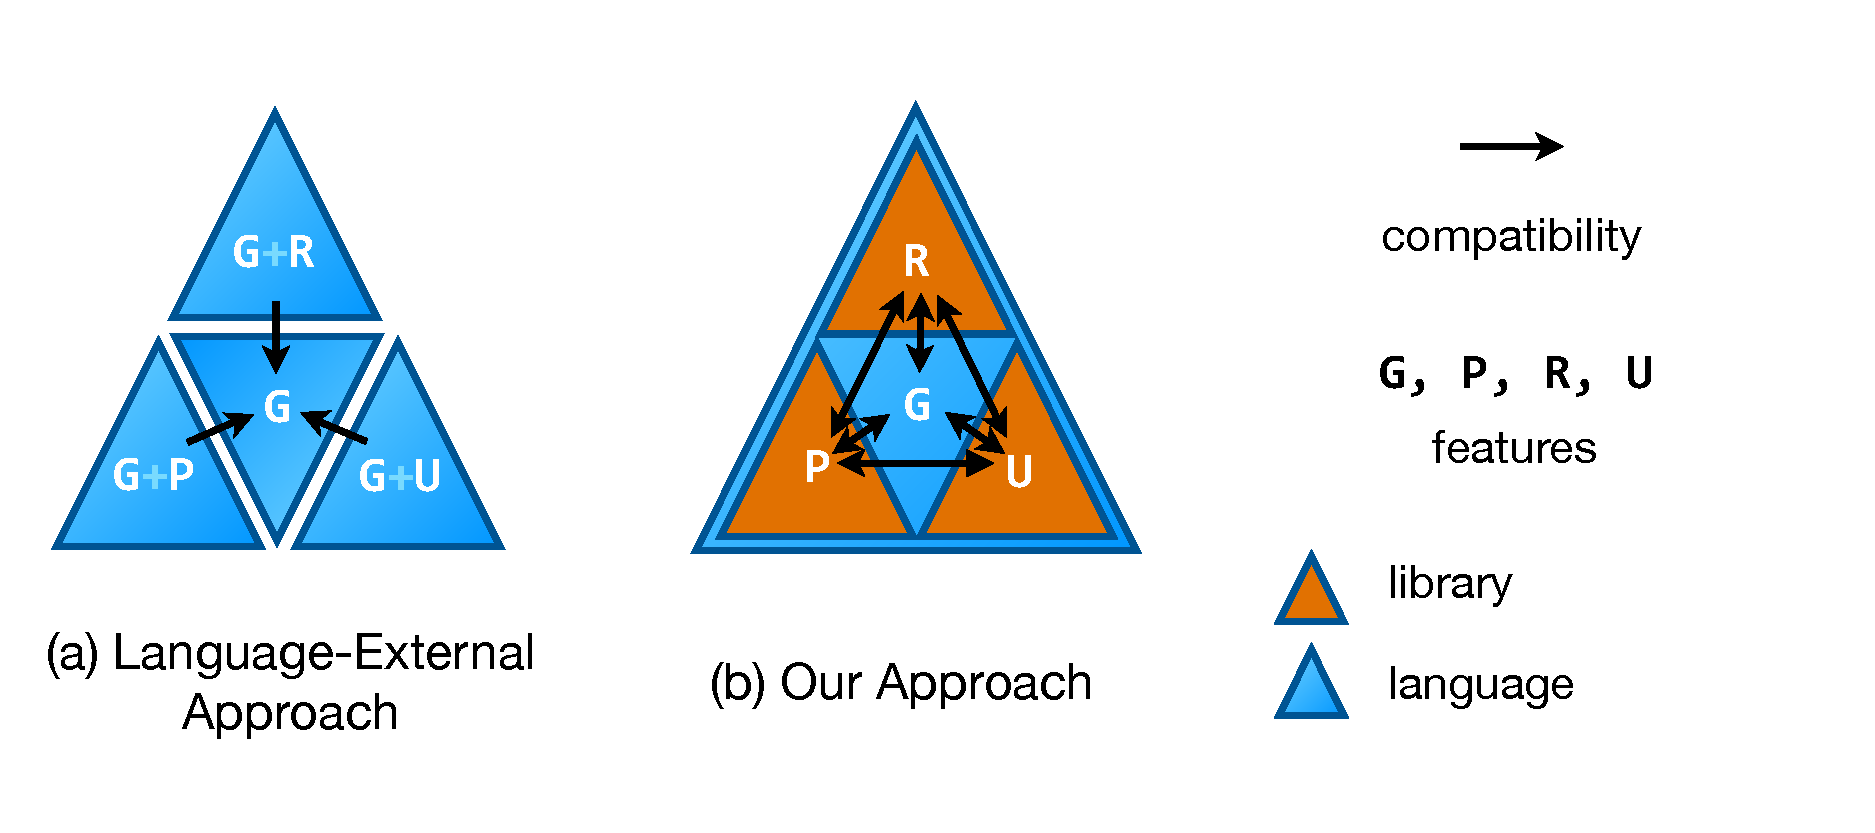
\includegraphics[scale=.48]{approaches.pdf}
% % \end{center}
% % \vspace{-20px}
% % \caption{\small (a) When taking a language-external approach, new features are packaged together into separate languages and tools. (b) We propose an approach where there is one extensible host language and the compile-time and edit-time logic governing new constructs is expressed within safely composable libraries.}
% % \label{approaches}
% % %\vspace{-10px}
% % \end{figure}
% %  %
% % % More specifically, there is no guarantee of \textbf{orthogonality} or even \textbf{interoperability}.% This has limited the broad adoption of these kinds of innovations.%This latter method couples the semantics of the feature to the implementation details of a particular tool. Because the use of one implementation entails a different semantics for the feature than another, the extended tool acts, \emph{de facto}, as a distinct system for our purposes. 

% % %\paragraph{Orthogonality} Features implemented by language-external means like these cannot be adopted individually, but instead are only available coupled to a fixed collection of other features. This makes adoption more costly when these incidental features are  not desirable or are insufficiently developed (``toy languages''), or when the features bundled with a different language or tool are simultaneously desirable. 

% % % Recent evidence indicates that this is one of the major barriers preventing research  from being driven into practice. For example, developers prefer high-level language-integrated parallel programming abstractions that provide  stronger semantic guarantees  \cite{cave2010comparing}, but library-based approximations are far more widely adopted because the ``parallel programming languages'' privilege only a few  specialized abstractions at the language level. In contrast, it is widely acknowledged that  different specialized abstractions are more appropriate in different situations \cite{Tasharofi:2013rc}. Moreover,  parallel programming is rarely the only relevant specialized concern. Support for regular expressions as above would be simultaneously desirable for processing large amounts of genomic data in parallel.% but using these features together in the same compilation unit would be difficult or impossible if implemented using language-external means. Indeed, switching to a ``parallel programming language'' would likely make it \emph{more} difficult to use regular expressions, as these are likely to be less well-developed in a specialized language than in an established general-purpose language.% This intuition was perhaps most succinctly expressed by a participant in a recent study by Basili et al. \cite{basili2008understanding}:  ``I hate MPI, I hate C++. [But] if I had to choose again, I would probably choose the same.'' %Similarly, a language and tools designed primarily to support regular expressions might make an interesting research project, but it would not be a suitable tool for writing large applications with more varied needs.

% % %\item Developing a new language and its associated tools places a significant development burden on providers who may wish only to promote a few core innovations, although tools like compiler generators, language workbenches and easy-to-extend tools can decrease this burden. 
% % %\item 

% % %Clients seem to prioritize the ability to choose different features for different portions of an application. 
% % %If calling between languages were safe and easy, then using a variety of specialized languages and associated tools might be less problematic. In fact, s
% % %Recognizing the limitations of relying on monolithic collection of primitives, some researchers have advocated instead for a model where multiple languages used within a single application, calling it the \emph{language-oriented approach} to software development \cite{languageoriented}. 

% % % \paragraph{Interoperability} Even in cases where, for each component of a software system, a programming system considered entirely satisfactory by its developers is available (e.g. a team goes through the trouble of implementing \verb|G+R+P| by reading papers about \verb|G+R| and \verb|G+P| and disentangling orthogonality-related issues), there remains a problem at any interface between  components written using a different combination of features. An interface that  externally exposes a specialized construct particular to one language (e.g. a function that requires a quantity having a particular unit of measure) cannot necessarily be safely and naturally consumed from another language (e.g. a parallel programming language). Tool support is also lost when calling into different languages. %We call this the \emph{interoperability problem}. % programs written by clients of a certain collection of features cannot always interface with programs written by clients of other features  in a safe, performant and natural manner.

% % % One strategy taken by proponents of a {language-oriented approach} \cite{journals/stp/Ward94} to partially address the interoperability problem is to  target an established intermediate language and use its constructs as a common language for communication between components written in different languages. Scala \cite{200464/IC} and F\# \cite{pickering2007foundations} are examples of prominent general-purpose languages that have taken this approach, and most DSL frameworks also rely on this strategy. As indicated in Figure \ref{approaches}a, this only enables interoperability in one direction. Calling into the common language becomes straightforward and safe, but calling in the other direction, or between the languages sharing the common target, does not, unless these languages are only trivially different from the common language. 

% % % %This approach only works well when new languages consist of constructs that can also be expressed safely and almost as naturally in the common language.
% % % %But many of the most innovative constructs found in modern languages (often, those that justify their creation) are difficult to define in terms of existing constructs in ways that guarantee all necessary invariants are statically maintained and that do not require large amounts boilerplate code and run-time overhead. 
% % % As a simple example with significant contemporary implications, F\#'s type system does not admit \verb|null| as a value for any type both defined and used within F\# code, but maintaining this sensible internal invariant still requires dynamic  checks because the stricter typing rules of F\# do not apply when F\# data structures are constructed by other languages on the Common Language Infrastructure (CLI) like C\# or SML.NET. This is not an issue exclusive to intermediate languages that make regrettable choices regarding \verb|null|, however. The F\# type system also includes support for checking that units of measure are used correctly \cite{syme2012expert, kennedy1994dimension}, but this more specialized static invariant is left entirely unchecked at language boundaries. Indeed, guidelines for F\# suggest that exposing functions that operate over values having units of measure, datatypes or tuples is not recommended when a component ``might be used'' from another language \cite{syme2012expert} because it is awkward to construct and consume these from other languages without the convenient primitive operations (e.g. pattern matching) and syntax that F\# includes. SML.NET prohibits exposing such types at component boundaries altogether. Moreover, it also cannot naturally consume F\# data structures, despite having a rather similar syntax and semantics in most ways (both languages directly descend from ML). 
% % %In Scala, traits that have default method implementations are difficult to implement from Java or other JVM languages and the workaround can break if the trait is modified \cite{scalatraitinterop}. 
% % %In some cases, desirable features must be omitted entirely due to concerns about interoperability. F\#, for example, aimed to retain source compatibility with Ocaml code, but due to the need for bidirectional interoperability with CLI languages, it does not support features like polymorphic variants, modules or functors \cite{ocaml-manual} because they have no apparent analogs in the type system of the CLI.
% % %\end{itemize}

% % %\subsection{Language-Integrated Approaches}\label{language-integrated-approaches}


% % %Such libraries have been called \emph{active libraries}  \cite{activelibraries}. %Features implemented within active libraries can be imported individually, unlike features implemented by external means, giving us a potential means to avoid the problems of orthogonality and interoperability just described.

% % % We must proceed with caution, however: critical issues having to do with {safety} must be overcome before language-integrated extension mechanisms can be introduced into a system. If too much control over  these core features of the system is given  to developers, the system's metatheory may become weak. 
% % % %For example, an extension could weaken important metatheoretic guarantees previously provided by the system. 
% % % For example, parsing ambiguities might arise if the syntax can be modified arbitrarily. Type safety  may not hold if the static and dynamic semantics of the language can be modified or extended arbitrarily from within libraries. Furthermore, even if extensions can be shown not to cause such problems in isolation, there may still be conflicts between extensions that could weaken their semantics, leading to subtle problems that only appear when two extensions are used together. %As a simple example, if two active libraries introduce the same syntactic form but back it with differing (but individually valid) semantics, this ambiguity  would only manifest itself when both libraries were imported within the same scope. %Resolving these kinds of ambiguities requires significantly more expertise with parser technology than using the syntax itself does. 
% % % These issues have plagued previous attempts to design language-integrated extensibility mechanisms.\todo{I can include a more detailed related work section if requested.}% We will briefly review some of these attempts below, then return to our approach.% To prevent them, our mechanisms will organize  extension logic around types to guarantee that extensions are both safe in isolation and also safely composable in any combination. 


% %  %This represents a minimalist approach to system design -- the conventional distinction between built-in and user-defined constructs is blurred and most features of the system are orthogonally implemented as {libraries}, rather than by the maintainers of the system.

% % %The mechanisms we describe will do so primarily by delimiting the scope of an extension to expressions of a single user-defined type or family of types. 

% % %This can be thought of as a more pernicious form of the conflict that arises when two globally-accessible constructs are given the same name. n languages without universal namespacing mechanisms (e.g. C, JavaScript, \LaTeX, ML and many others). 

% % %The extension mechanism\todo{elaborate on safety requirements + tension between expressiveness and safety, merge with next paragraph}. must be expressive enough to allow users to associate rich run-time, compile-time and edit-time behaviors with user constructs directly, while being sufficiently restrictive to maintain the global safety properties of the language and system as a whole, and to ensure that constructs cannot interfere with one another. 
